\documentclass[10pt,aspectratio=169]{beamer}

\usetheme[progressbar=frametitle]{metropolis}

\title{Mathematical Foundations of Computer Science}
\subtitle{Decidability of string graphs}
\date{26.01.2023}
\author{Pavel Zwerschke}
\institute{Radboud University Nijmegen}
\titlegraphic{\hfill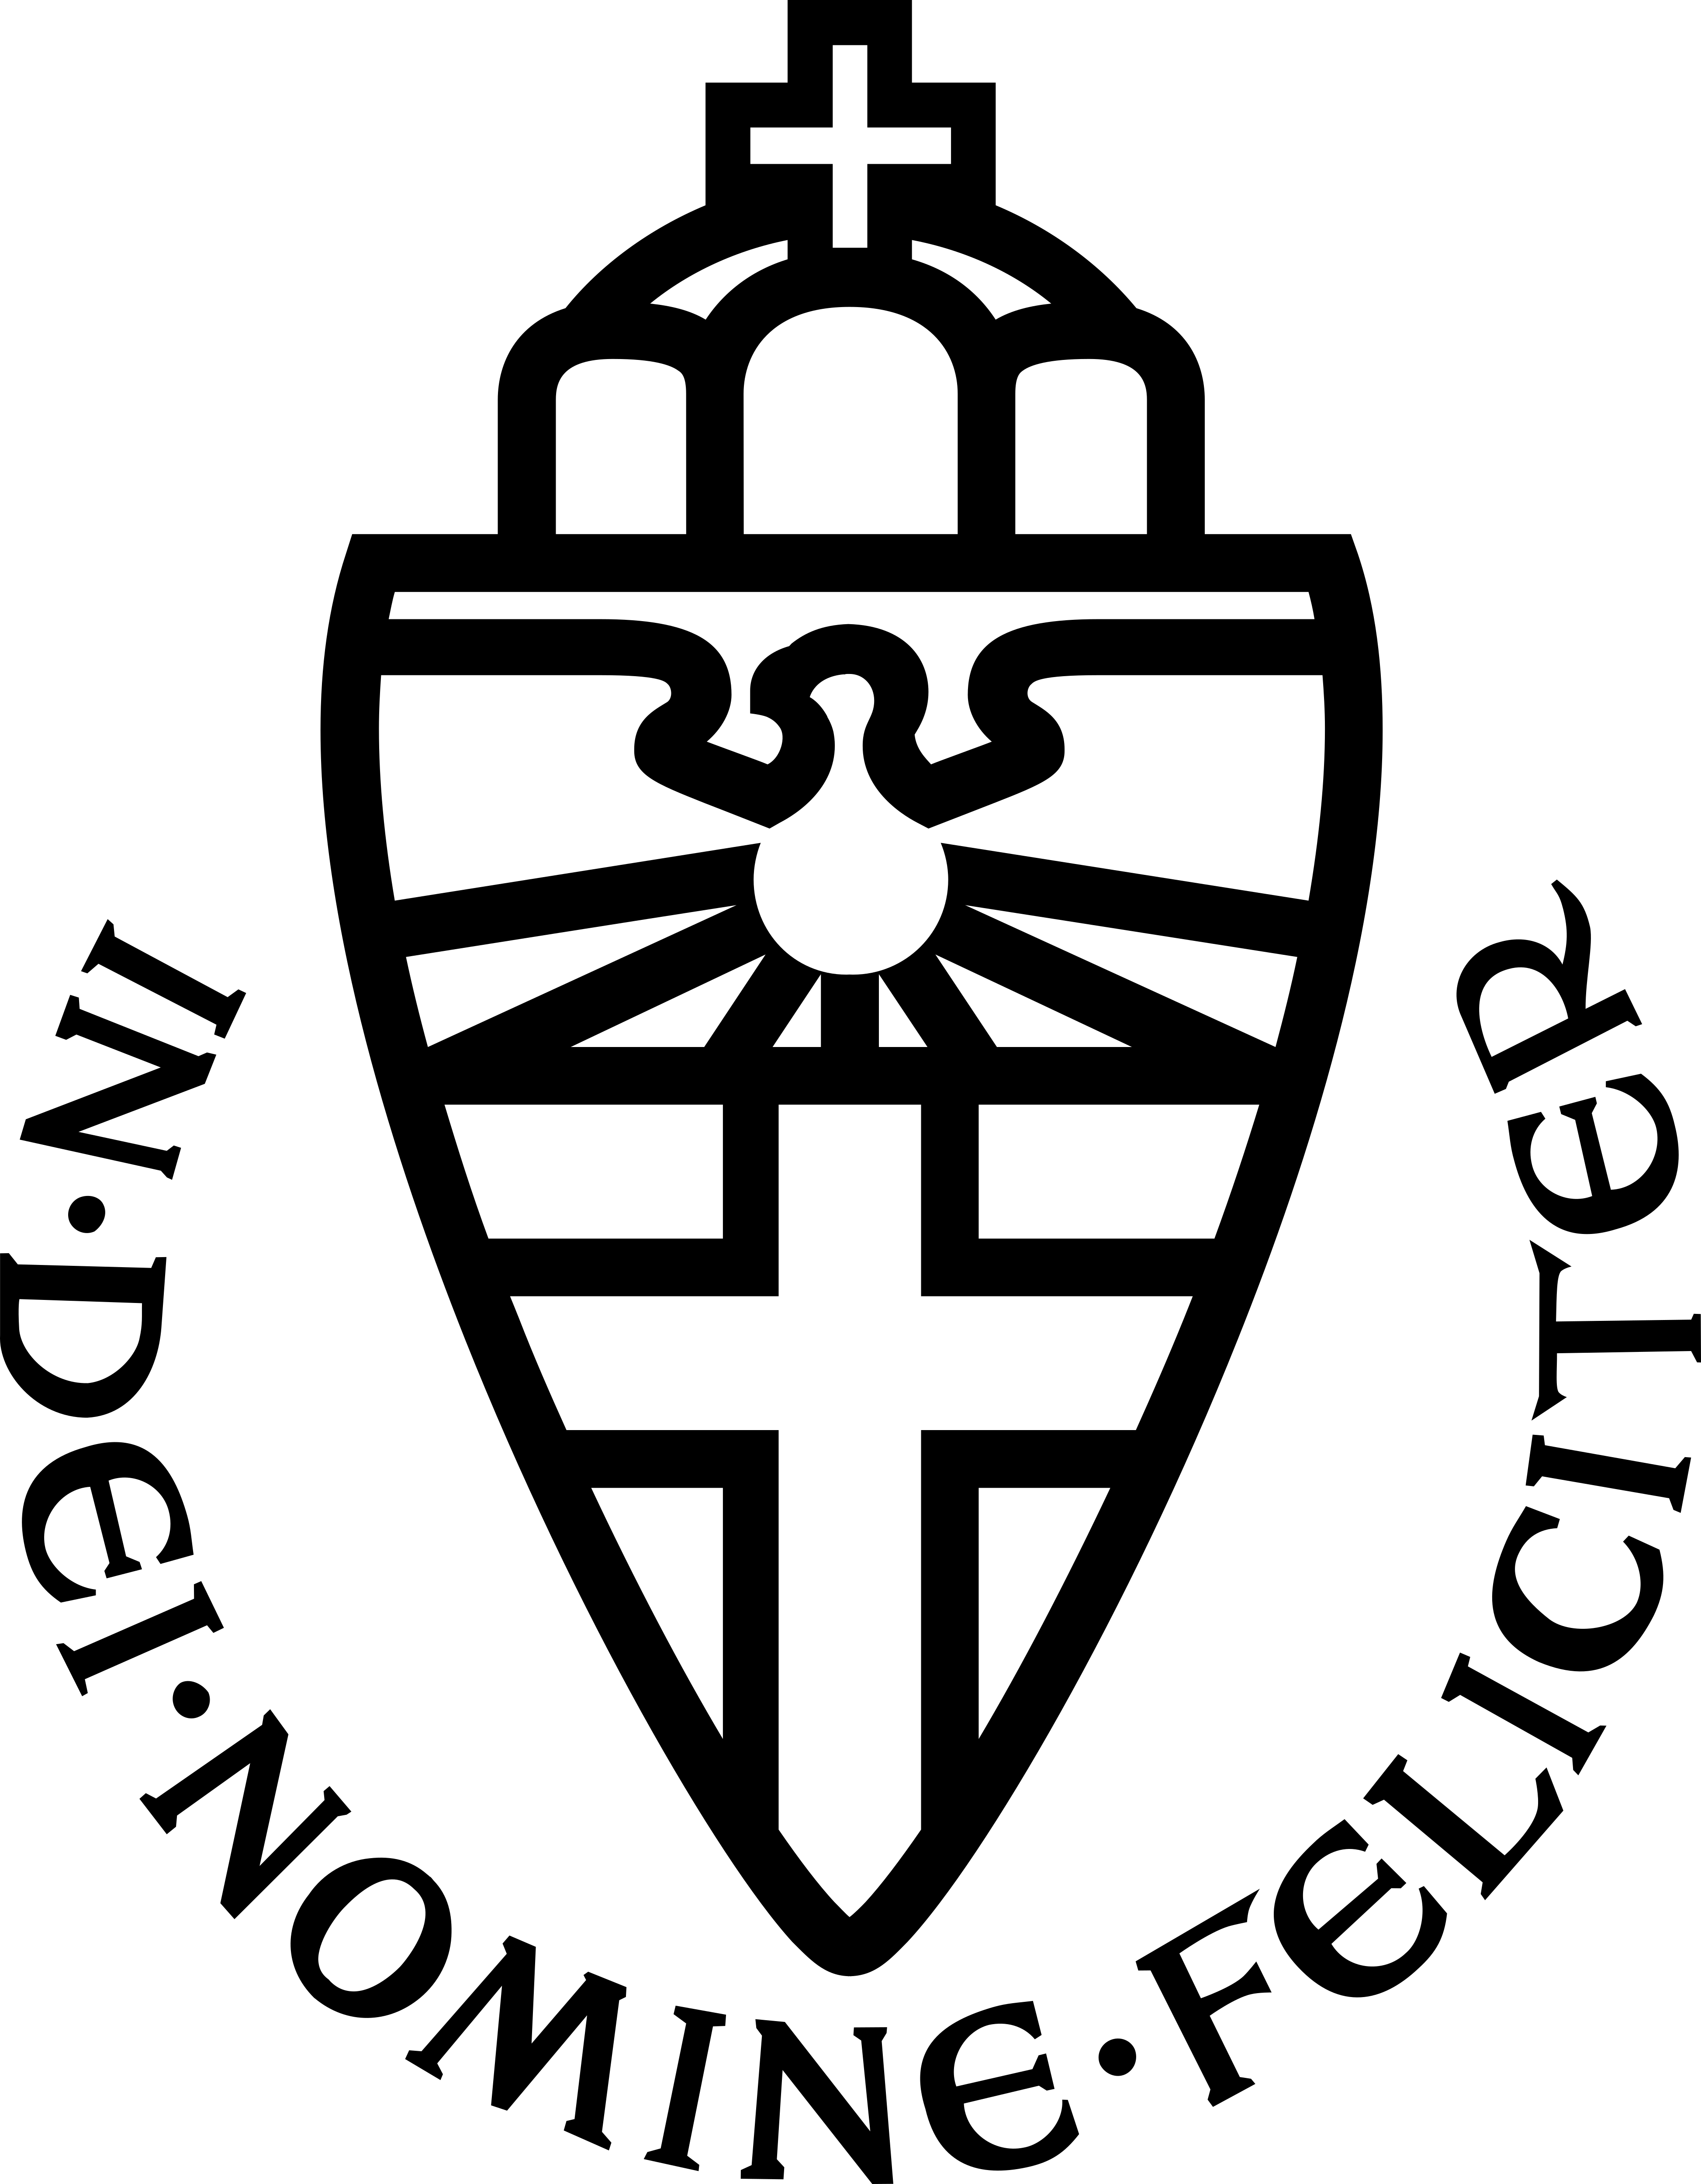
\includegraphics[height=1.5cm]{logos/radboud-university}}

% BibTeX setup
% \usepackage[backend=bibtex, bibstyle=alphabetic, citestyle=alphabetic]{biblatex}
% \bibliography{references}

\usepackage[english]{babel} % English

% Standard packages for math-related things.
\usepackage{amsmath}
\usepackage{amssymb}
\usepackage{amsthm}
\usepackage{mathtools}

\usepackage{graphicx} % to include graphics with \includegraphics[options]{imagefile}

\theoremstyle{plain} % Usual style for theorems, etc.

\setbeamertemplate{theorems}[numbered]

\theoremstyle{remark} % Usual style definitions.
\newtheorem{remark}[theorem]{Remark}

\newcommand{\N}{\mathbb{N}}
\newcommand{\R}{\mathbb{R}}
\newcommand{\Z}{\mathbb{Z}}

\newcommand{\set}[1]{\{#1\}}
\newcommand{\norm}[1]{\|#1\|}

\begin{document}

\maketitle

% \begin{frame}{Table of contents}
%     \setbeamertemplate{section in toc}[sections numbered]
%     \tableofcontents%[hideallsubsections]
% \end{frame}

\section{Introduction}

\begin{frame}{What is a string graph?}
    \setbeamertemplate{background}[grid]
    \begin{itemize}
        \item A \textit{curve} (or \textit{string}) is a set homeomorphic to \([0,1]\)
        \item Given a collection of curves \((C_i)_{i \in I}\) in the plane, the corresponding intersection graph is \( (I, \set{\set{i, j} : C_i \text{ and } C_j \text{ intersect}}) \)
        \item \textit{string graph}: a graph isomorphic to the intersection graph of a collection of curves 
    \end{itemize}
\end{frame}

\begin{frame}{Non-string graph example}
    There are graph instances that cannot be string graphs.

    \begin{center}
        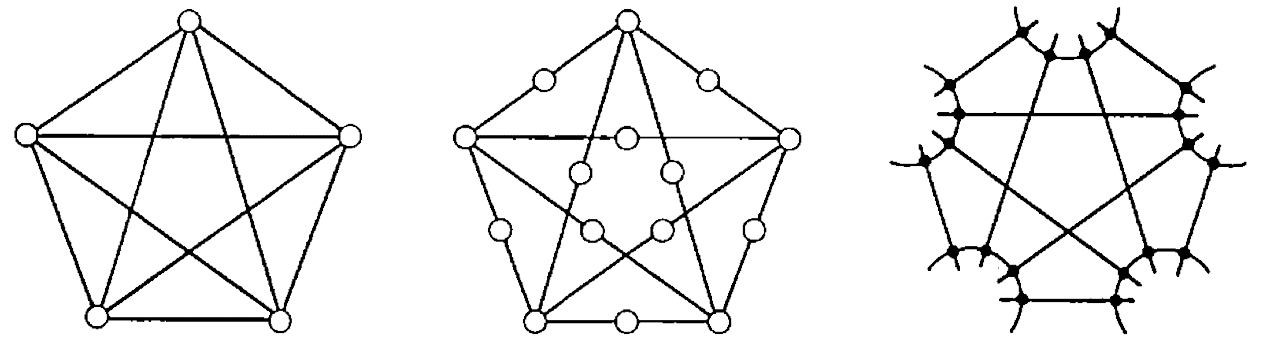
\includegraphics[width=0.8\textwidth]{images/figure-0.png}
    \end{center}
\end{frame}

\begin{frame}{Definitions}
    \begin{itemize}
        \item \textit{size} of a collection of curves: the number of intersection points
        \item \(c_s(G)\): the size of the smallest (smallest number of intersections) set of curves whose intersection graph is isomorphic to \(G\)
        \item Define \(c_s(m) = \max\set{c_s(G) : G \text{ has } m \text{ edges}}\)
    \end{itemize}
\end{frame}

\begin{frame}{\(c_s(G)\) is finite}
    \begin{itemize}
        \item It is not obvious that \(c_s(G)\) is finite for every string graph \(G\)
        \item Kratochvíl et al. showed that \(c_s(G)\) is finite for every string graph \(G\)
    \end{itemize}
    \begin{lemma}
        A string graph can be realized by a family of polygonal arcs with a finite number of intersections.
        \label{lem:finite-cs}
    \end{lemma}
\end{frame}

\setbeamertemplate{background}[grid]
\addtocounter{theorem}{-1}
\begin{frame}[t]{Lemma \ref{lem:finite-cs} Proof}
    \begin{lemma}
        A string graph can be realized by a family of polygonal arcs with a finite number of intersections.
    \end{lemma}
\end{frame}
\setbeamertemplate{background}[default]

\begin{frame}{Realizability}
    \begin{itemize}
        \item Graph \(G = (V, E)\), \(R \subseteq \binom{E}{2} = \set{\set{e, f} : e, f \in E} \) on \(E\)
        \item call a drawing \(D\) of \(G\) in the plane a \textit{weak realization} of \((G, R)\) if only pairs of edges which are in \(R\) are allowed to intersect in \(D\)
        \item call a drawing \(D\) of \(G\) in the plane a \textit{realization} of \((G, R)\) if exactly pairs of edges which are in \(R\) are intersect in \(D\)
        \pause
        \item \(c_w(G, R)\) is the smallest number of intersections in a weak realization of \((G, R)\)
        \item \(c_w(G) = \max\set{c_w(G, R) : (G, R) \text{ has a weak realization}} \)
        \item \(c_w(m) = \max\set{c_w(G) : G \text{ has } m \text{ edges}}\)
        \item Define \(c_r(G, R)\), \(c_r(G)\) and \(c_r(m)\) similarly for realizations
        \pause
        \item \(\mathrm{cr}(G) = c_w(G, \binom{E}{2})\) is known as the crossing number (\(\mathbf{NP}\)-complete)
        \item \(c_w(G, \emptyset)\) is equivalent to planarity testing (in \(\mathbf{P}\))
    \end{itemize}
\end{frame}

\begin{frame}{Relationships between realizability functions}
    \begin{lemma}
        \(c_r\), \(c_w\) and \(c_s\) are polynomially equivalent.
        \label{lem:pol-equivalent}
    \end{lemma}
\end{frame}

\setbeamertemplate{background}[grid]
\addtocounter{theorem}{-1}
\begin{frame}[t]{Lemma \ref{lem:pol-equivalent} Proof}
    \begin{lemma}
        \(c_r\), \(c_w\) and \(c_s\) are polynomially equivalent.
    \end{lemma}
\end{frame}
\setbeamertemplate{background}[default]

\section{Bounding the Number of Intersections}

\begin{frame}{Bounding the Number of Intersections -- Strategy}
    Show by contradiction: There exists a drawing for a realizability problem 
    s.t. there are \(< 2^m\) intersections for each edge \(e\) in \(D\).\pause

    This gets translated into a string graph problem with Lemma \ref{lem:pol-equivalent}.\pause

    Every string graph must have a representation with maximally exponential size.\pause

    Construct an algorithm to check if something is a string graph in \(\mathbf{NEXP}\).
\end{frame}

\begin{frame}{Bounding the Number of Intersections 1}
    Assign each curve a unique number \(\leadsto\) intersections along a particular curve is a word over an alphabet
    \begin{lemma}
        Every word of length \(\geq 2^n\) over an alphabet of size \(n\) contains a non-trivial subword in which every character occurs an even number of times.
        \label{lem:even-occurrences}
    \end{lemma}
\end{frame}

\setbeamertemplate{background}[grid]
\addtocounter{theorem}{-1}
\begin{frame}[t]{Lemma \ref{lem:even-occurrences} Proof}
    \begin{lemma}
        Every word of length \(\geq 2^n\) over an alphabet of size \(n\) contains a non-trivial subword in which every character occurs an even number of times.
    \end{lemma}
\end{frame}
\setbeamertemplate{background}[default]

\begin{frame}{Lemma \ref{lem:even-occurrences} Example}
    \(w = 12312231, |w| = 8 \geq 2^3\)

    \[ v_0 = \begin{pmatrix}
    0 \\ 0 \\ 0
    \end{pmatrix}, v_1 = \begin{pmatrix}
    1 \\ 0 \\ 0
    \end{pmatrix}, v_2 = \begin{pmatrix}
    1 \\ 1 \\ 0
    \end{pmatrix}, v_3 = \begin{pmatrix}
    1 \\ 1 \\ 1
    \end{pmatrix}, v_4 = \begin{pmatrix}
    0 \\ 1 \\ 1
    \end{pmatrix}, \]
    
    \[ v_5 = \begin{pmatrix}
    0 \\ 0 \\ 1
    \end{pmatrix}, v_6 = \begin{pmatrix}
    0 \\ 1 \\ 1
    \end{pmatrix}, v_7 = \begin{pmatrix}
    0 \\ 1 \\ 0
    \end{pmatrix}, v_8 = \begin{pmatrix}
    1 \\ 1 \\ 0
    \end{pmatrix} \]
\end{frame}

\begin{frame}{Bounding the Number of Intersections 2}
    \begin{theorem}
        Let \(G\) be a graph with \(m\) edges, \(R \subseteq \binom{E}{2}\) such that \((G, R)\) is weakly realizable, and let \(D\) 
        be a weak realization of \((G, R)\) with the minimal number of intersections. Then for any edge \(e \in G\) 
        there are less than \(2^m\) intersections on the curve realizing \(e\) in \(D\).
    \end{theorem}
\end{frame}

\begin{frame}{Bounding the Number of Intersections 3}
    \begin{columns}
    \begin{column}{0.35\textwidth}
        \begin{itemize}
            \item Suppose not. Let \(D\) be a weak realization of \((G, R)\) with minimal number of intersections.
            \item<2-> Let \(e\) be an edge which has \(> 2^m - 1\) intersections.
            \item<3-> Choose a segment of \(e\) which is intersected an even number of times by any other edge. Draw a window around this segment with no other intersections.
        \end{itemize}
    \end{column}
    \begin{column}{0.65\textwidth}
        \begin{center}
            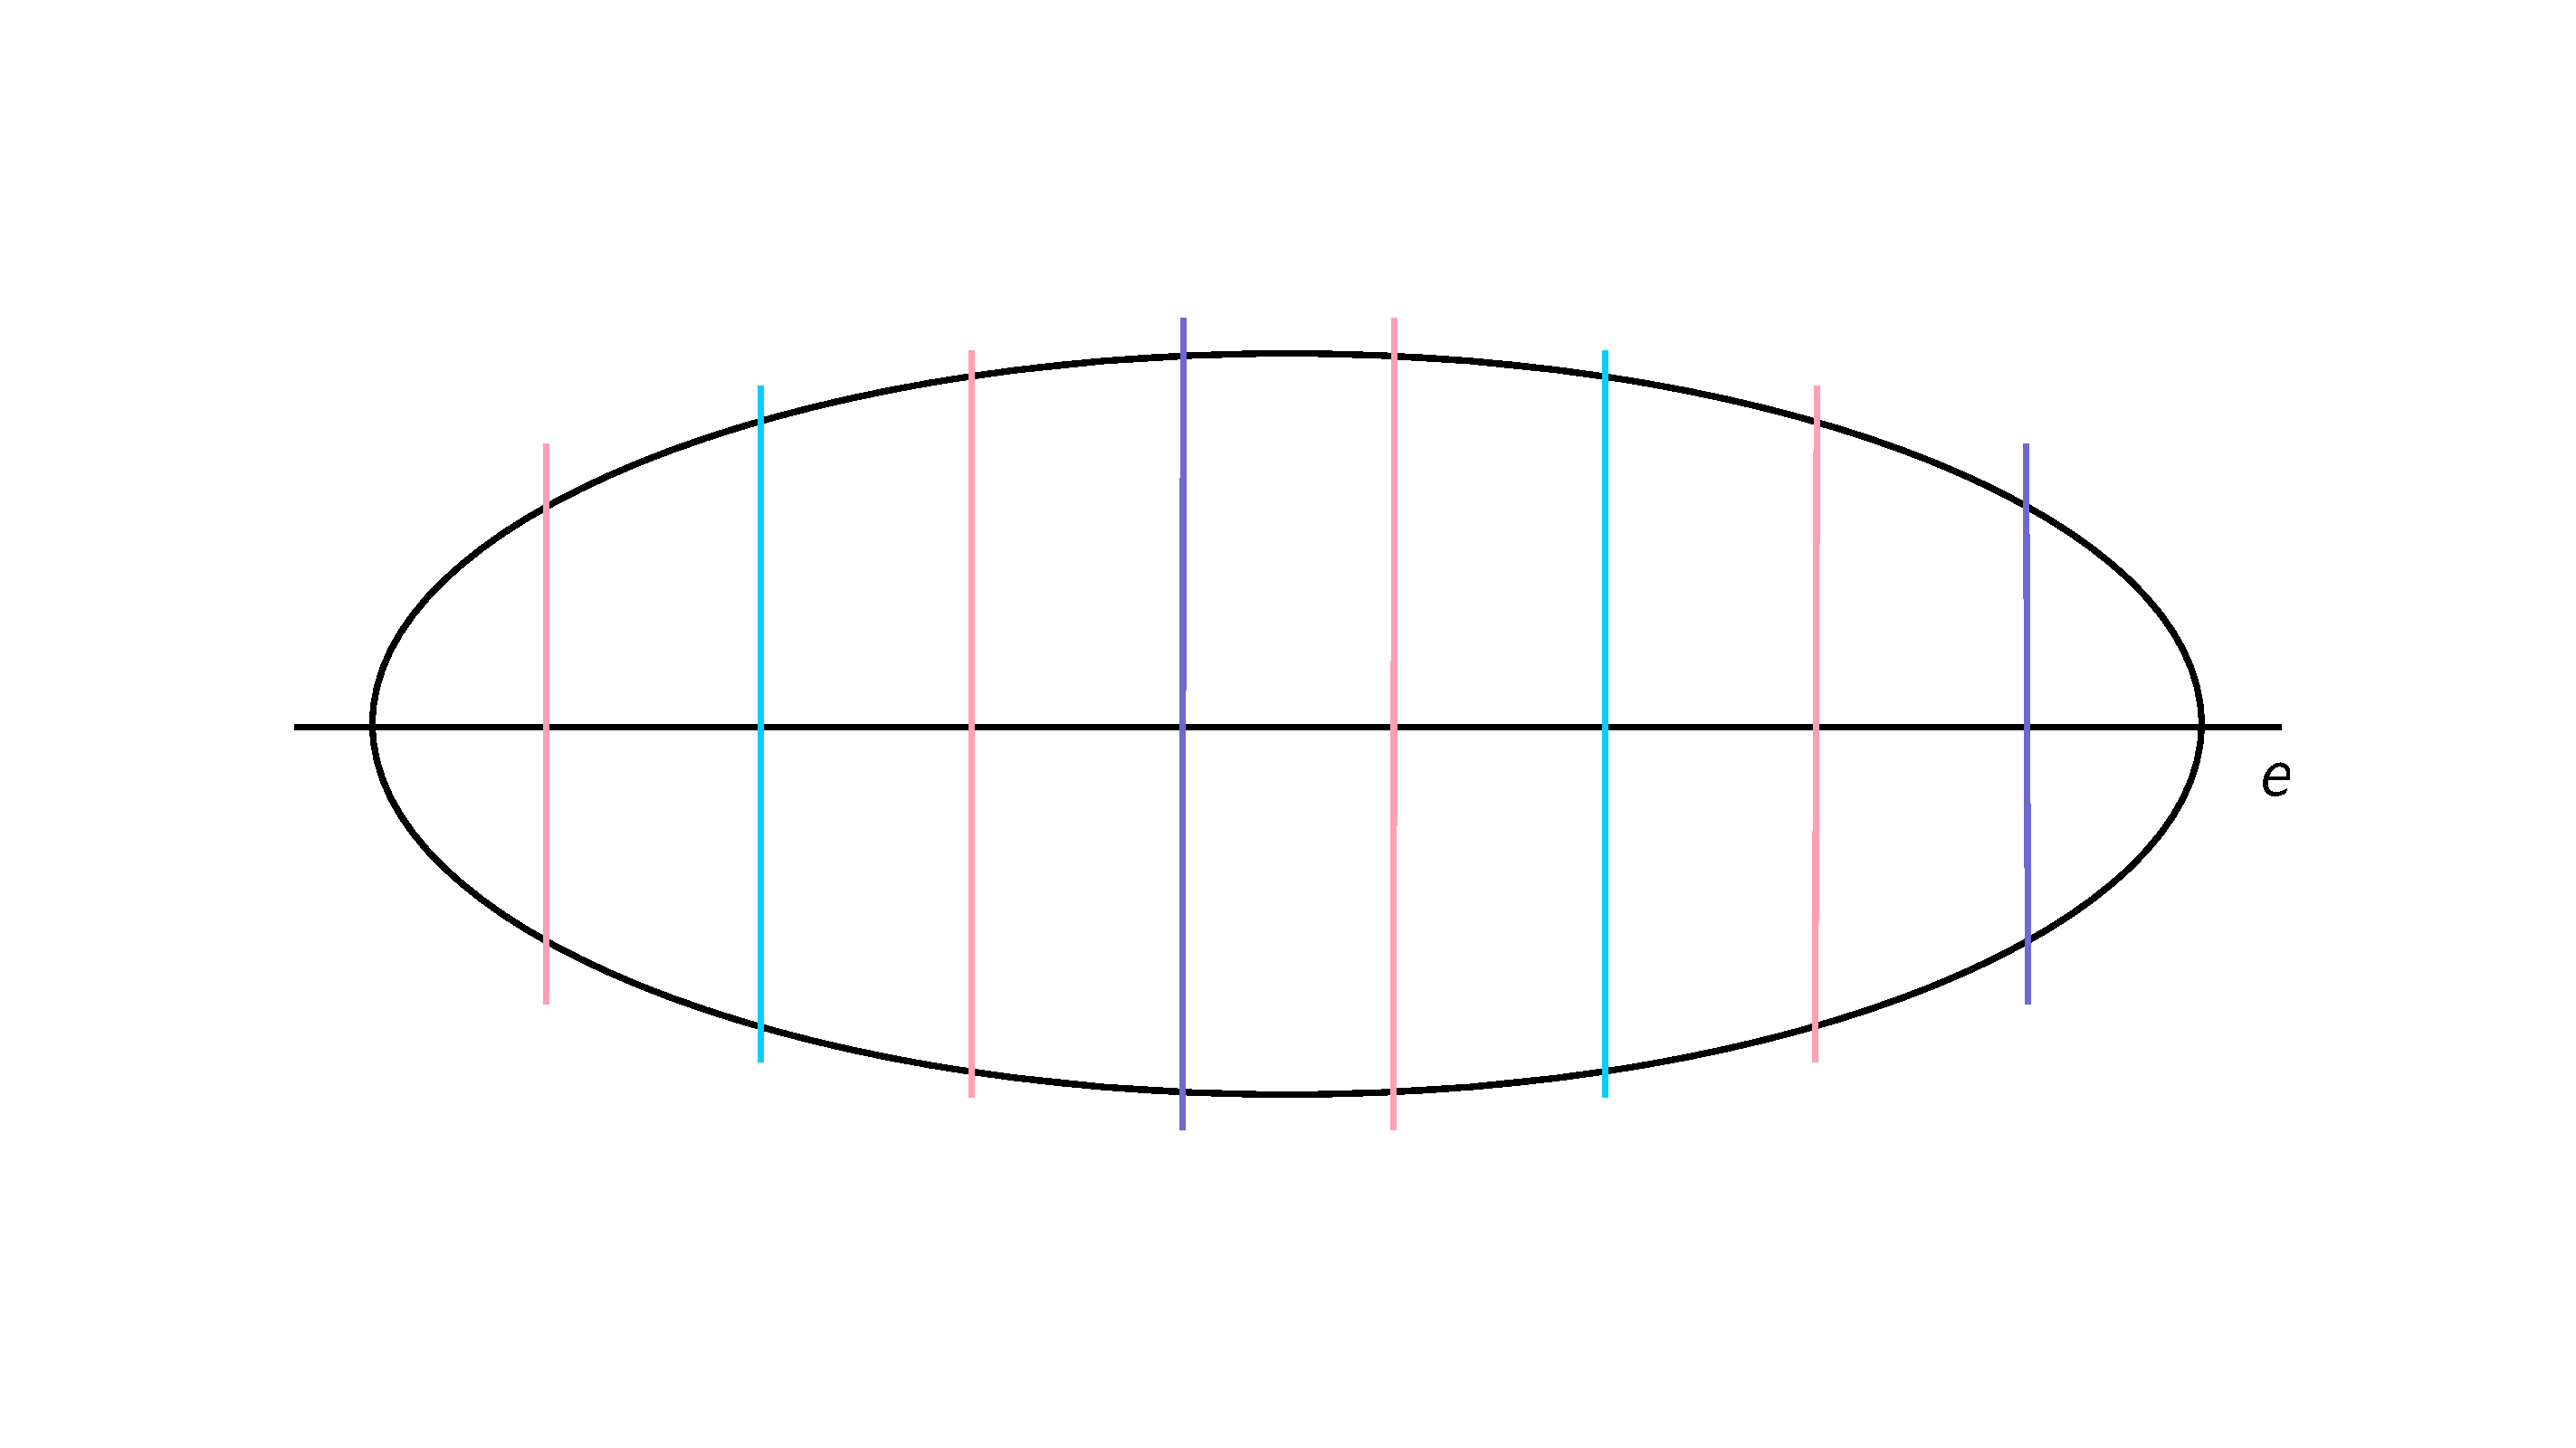
\includegraphics[width=\textwidth]{images/figure-4.pdf}
        \end{center}
    \end{column}
    \end{columns}
\end{frame}

\begin{frame}{Bounding the Number of Intersections 4}
    \begin{columns}
    \begin{column}{0.35\textwidth}
        \begin{itemize}
            \item Let \(2n_f\) be the number of intersections of edge \(f\) with \(e\) in this window.
            \item<2-> For each \(f\), assign numbers \(1, \ldots, 4 n_f\) to the intersections with the window in the order they appear on \(f\).
            \item<3-> We can assume (by Jordan-Schoenflies theorem) that the window is a circle and \(e\) is a straight line and \(\forall f\), the intersections \(2i-1\) and \(2i\) are mirror images.
        \end{itemize}
    \end{column}
    \begin{column}{0.65\textwidth}
        \begin{center}
            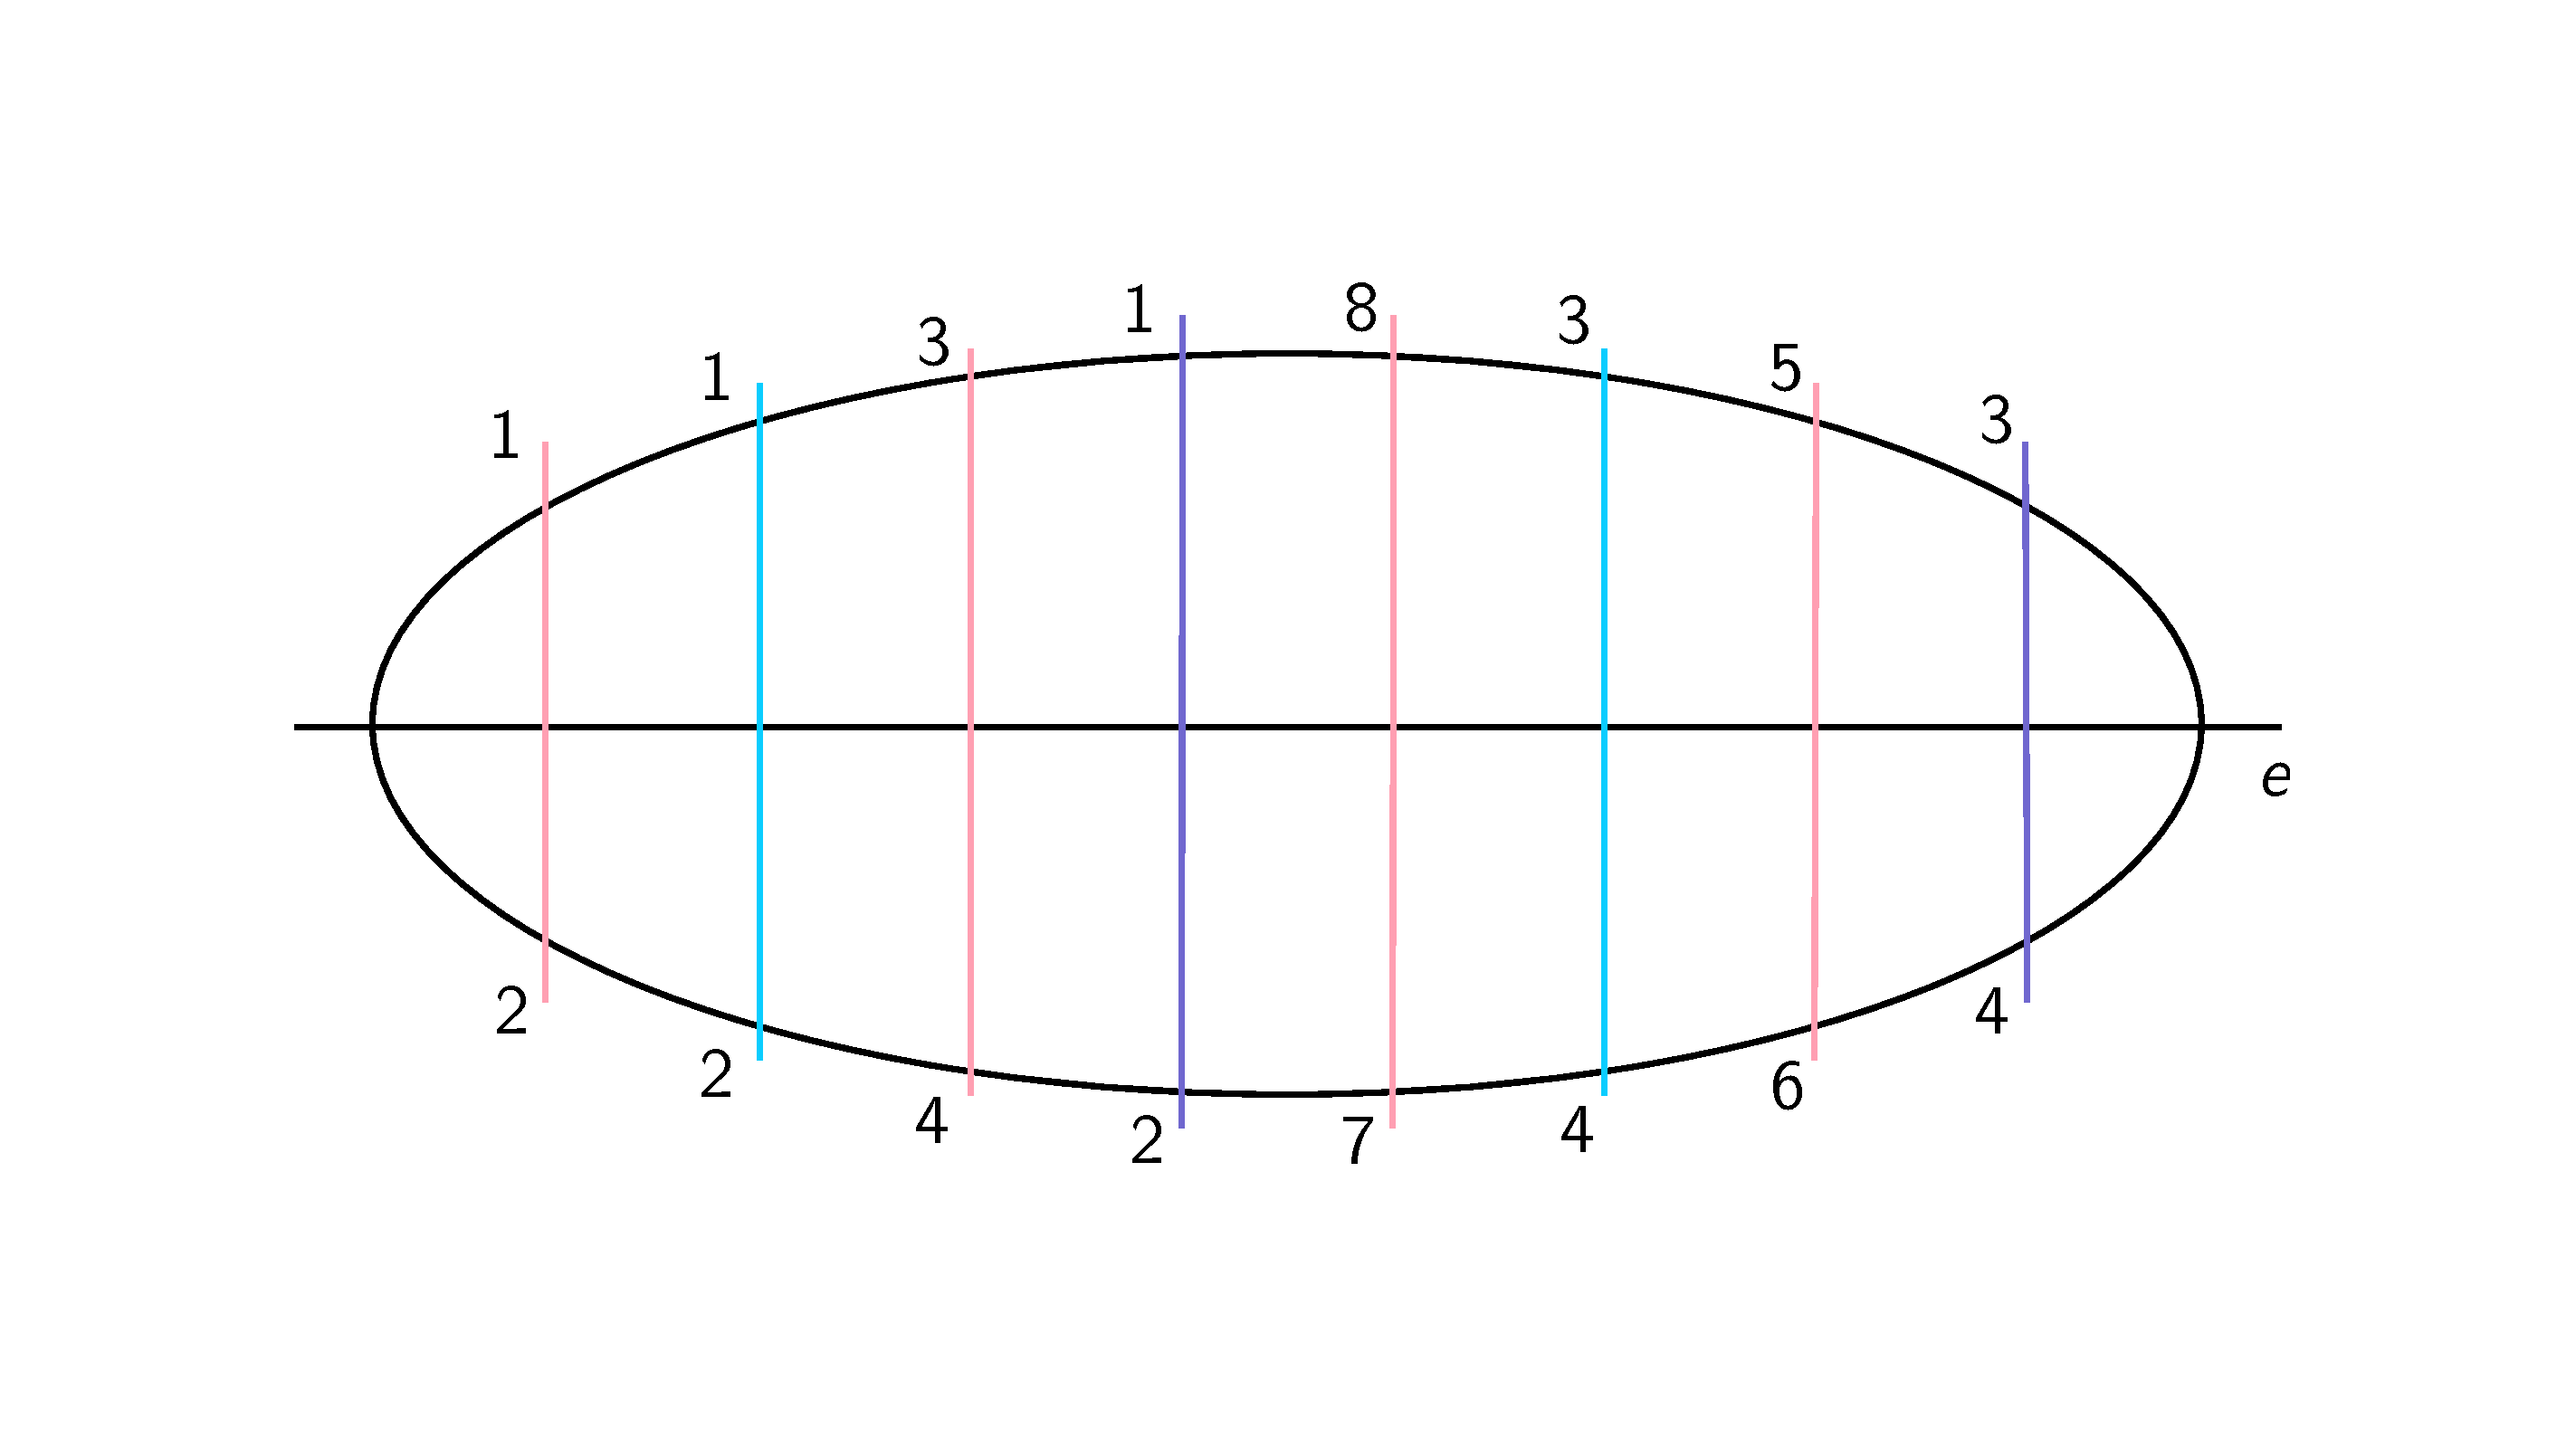
\includegraphics[width=\textwidth]{images/figure-5.pdf}
        \end{center}
    \end{column}
    \end{columns}
\end{frame}

\begin{frame}{Bounding the Number of Intersections 5}
    \begin{columns}
    \begin{column}{0.35\textwidth}
        \begin{itemize}
            \item For each \(f\), there is a connection between \(4i-2\) and \(4i-1\) lying completely outside the window.
        \end{itemize}
    \end{column}
    \begin{column}{0.65\textwidth}
        \begin{center}
            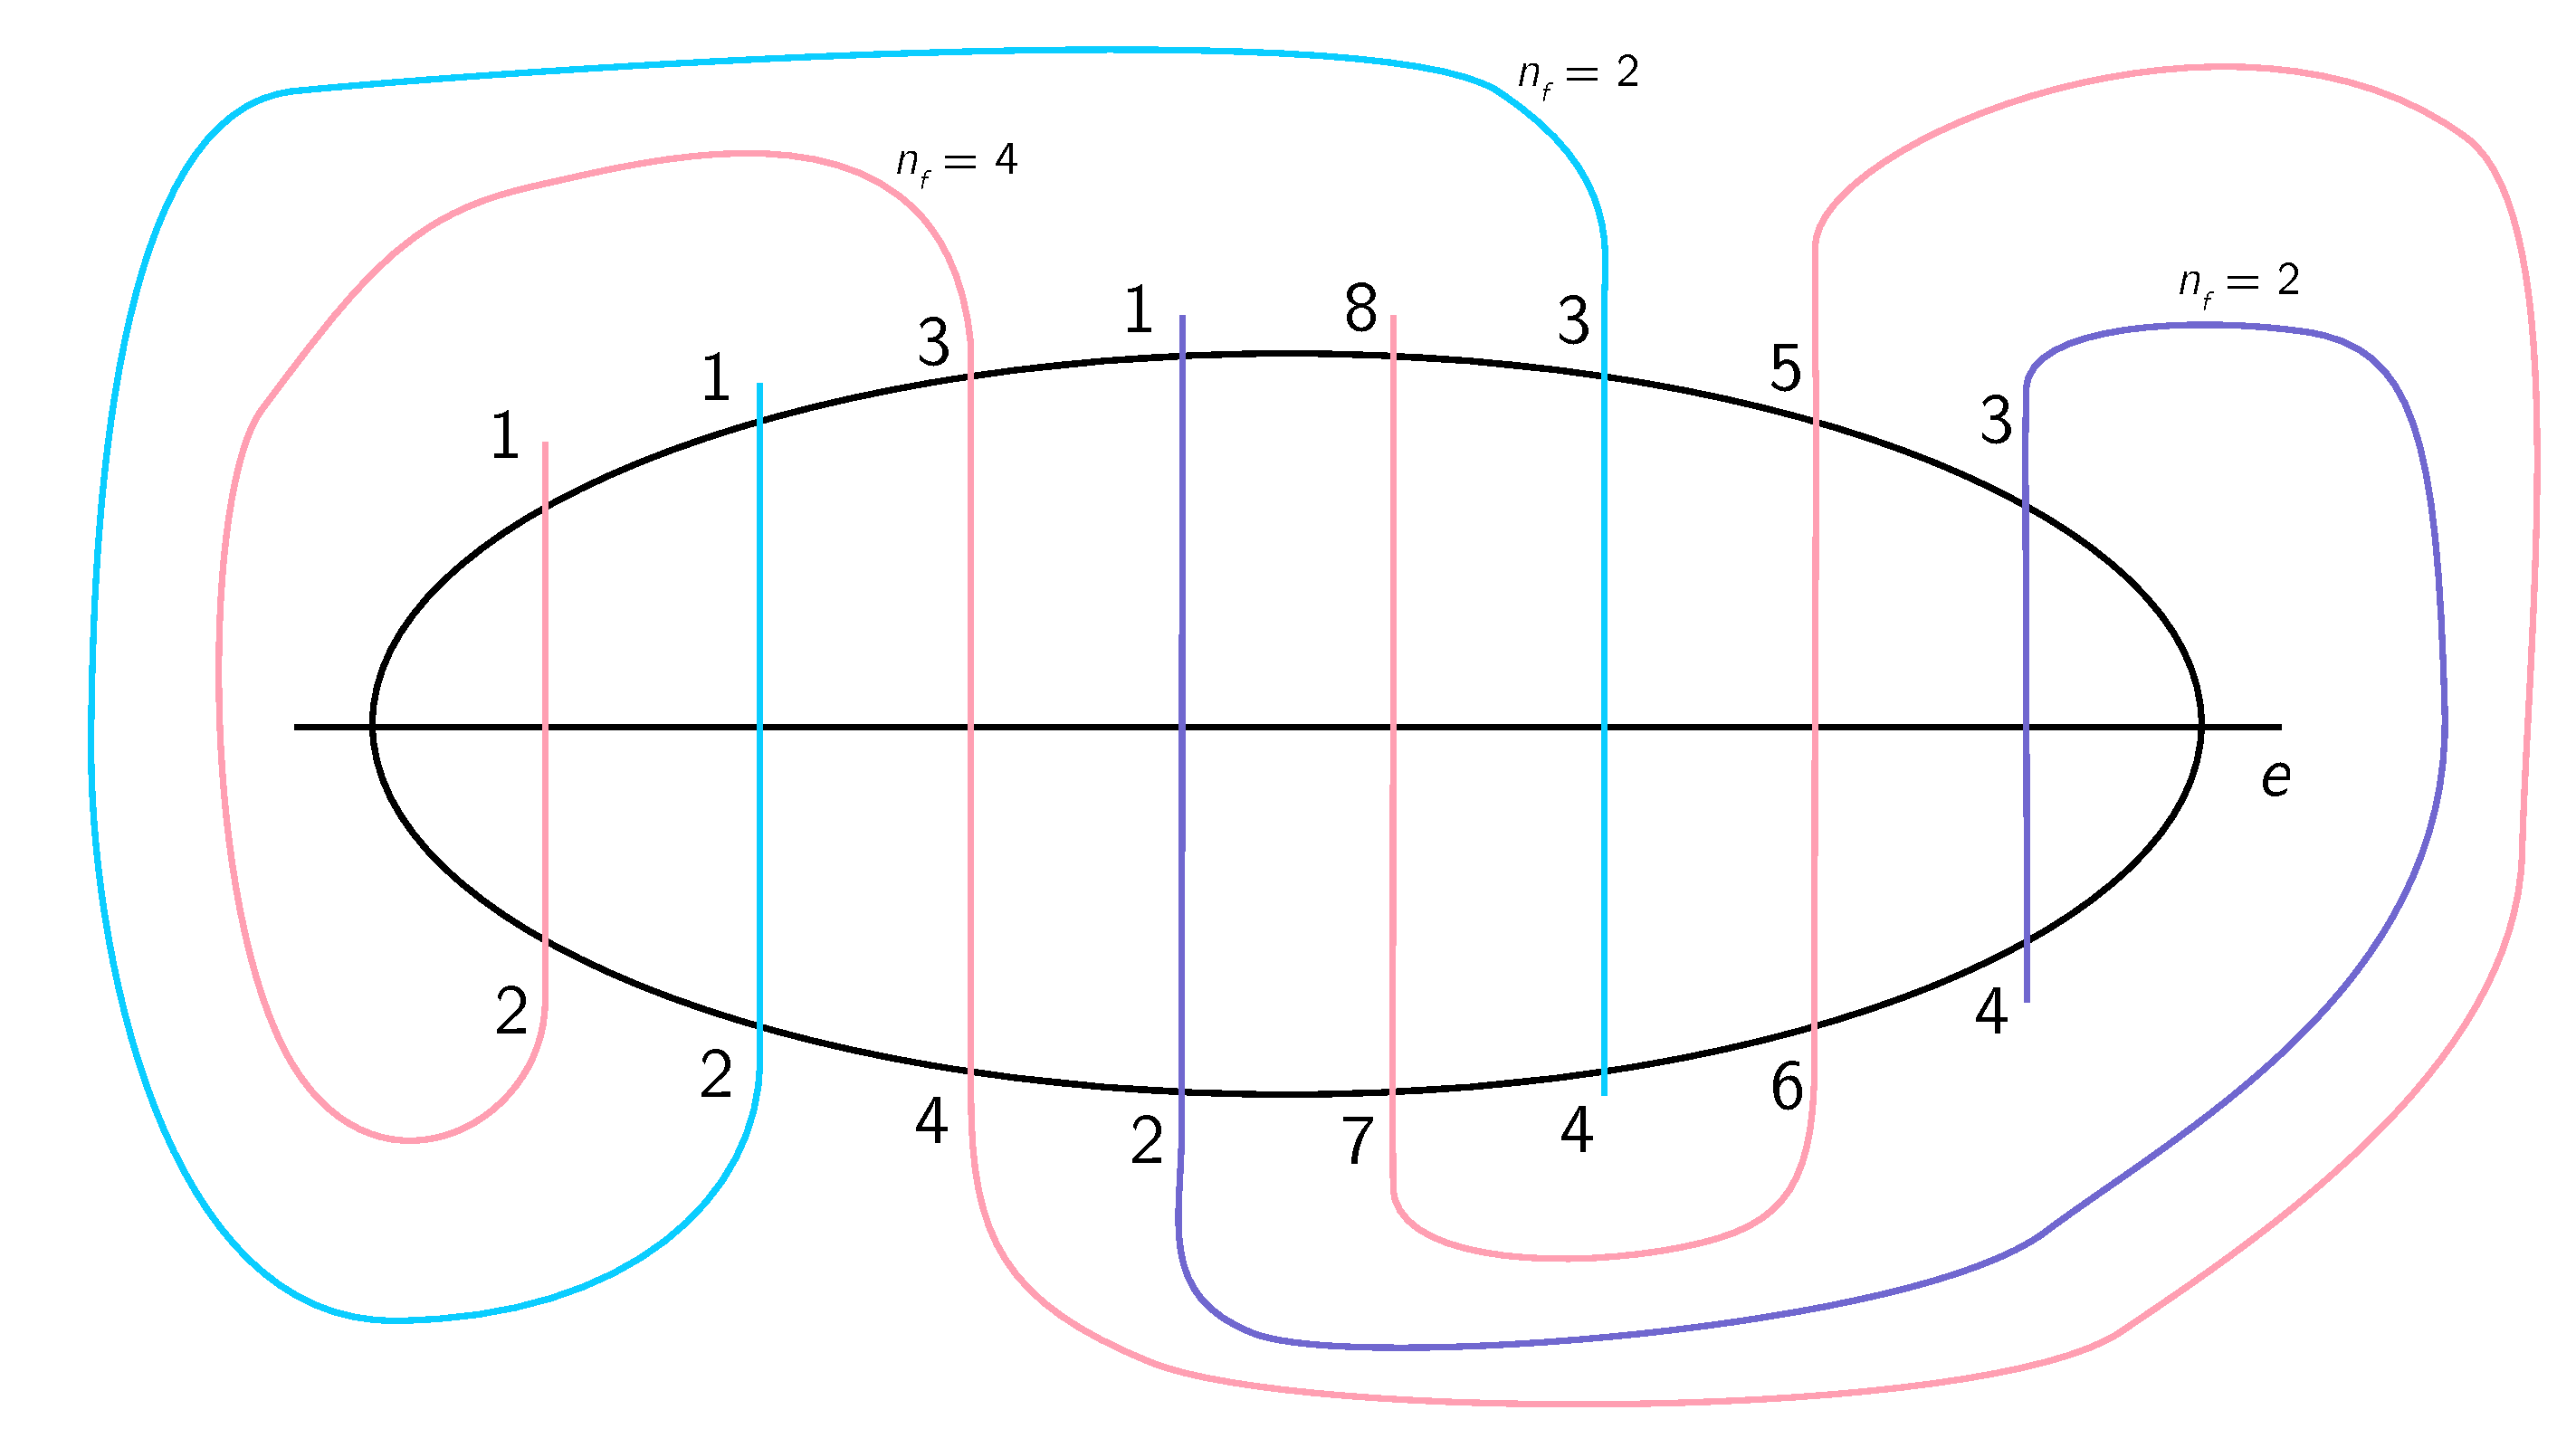
\includegraphics[width=\textwidth]{images/figure-6.pdf}
        \end{center}
    \end{column}
    \end{columns}
\end{frame}

\begin{frame}{Bounding the Number of Intersections 6}
    \begin{columns}
    \begin{column}{0.35\textwidth}
        \begin{itemize}
            \item Use circular inversion along the circle to bring all of these conections inside.
        \end{itemize}
    \end{column}
    \begin{column}{0.65\textwidth}
        \begin{center}
            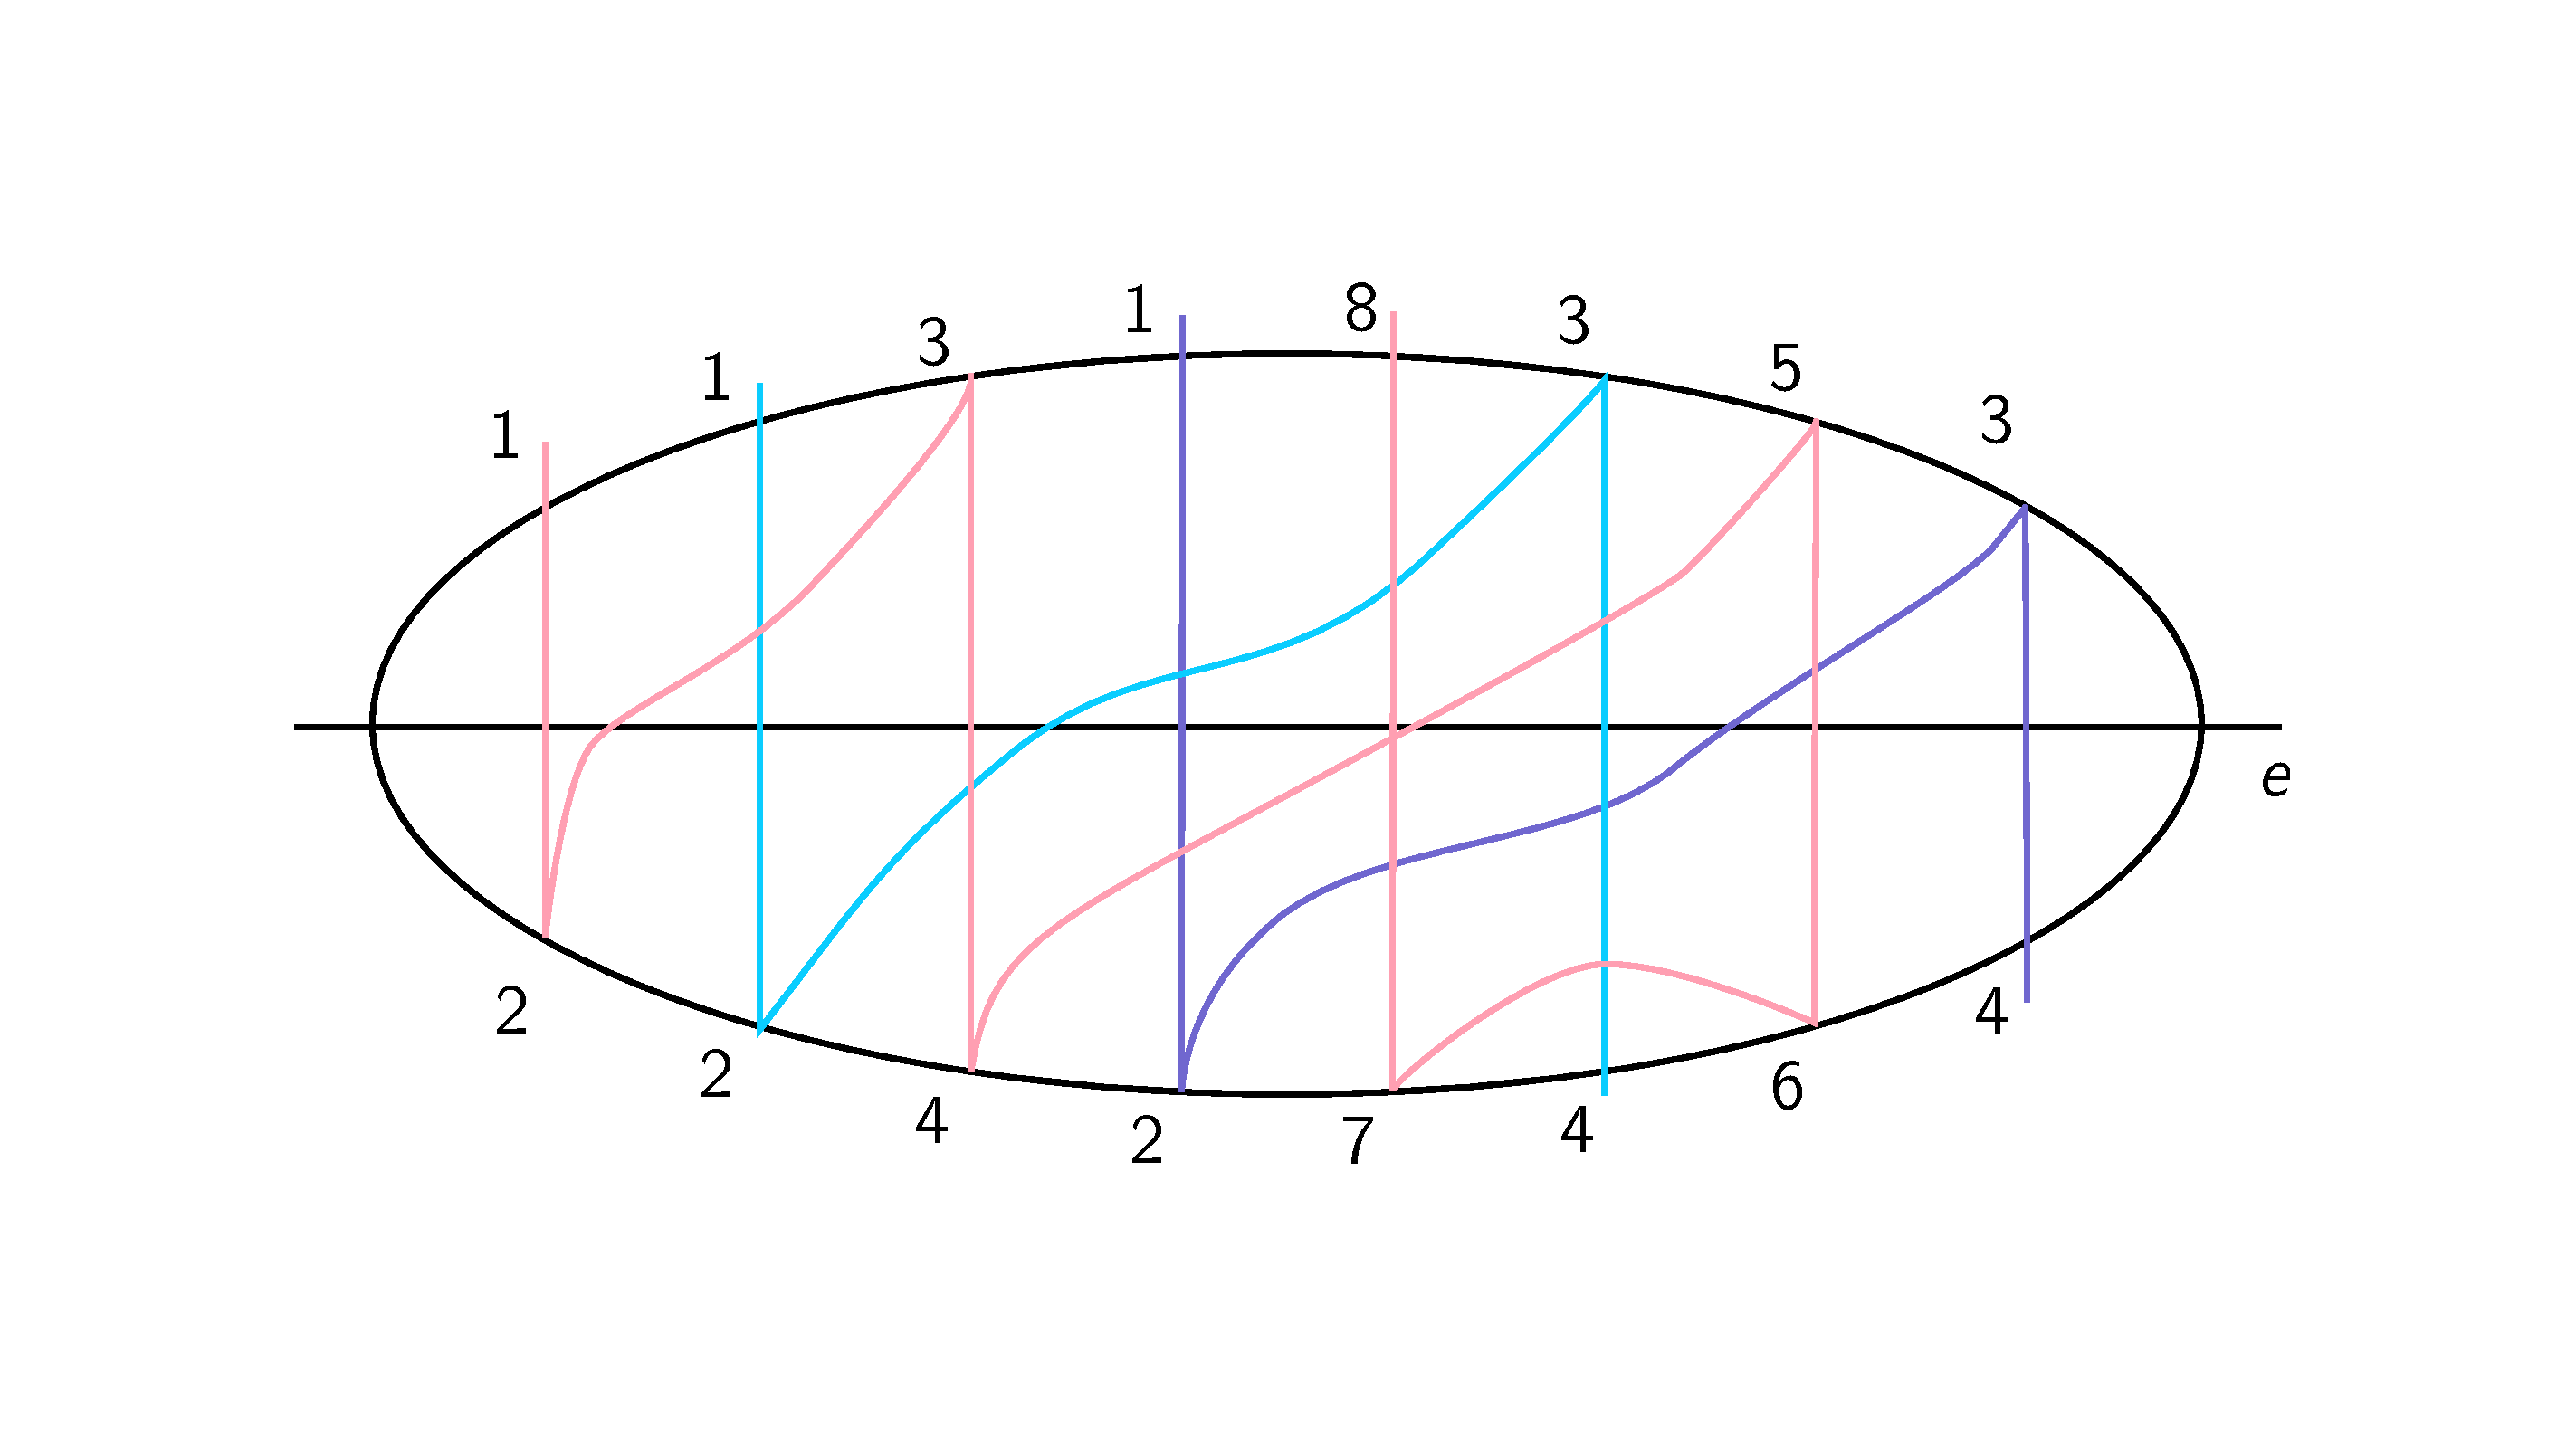
\includegraphics[width=\textwidth]{images/figure-7.pdf}
        \end{center}
    \end{column}
    \end{columns}
\end{frame}

\begin{frame}{Bounding the Number of Intersections 7}
    \begin{columns}
    \begin{column}{0.35\textwidth}
        \begin{itemize}
            \item Mirror everything inside of the window along \(e\).
        \end{itemize}
    \end{column}
    \begin{column}{0.65\textwidth}
        \begin{center}
            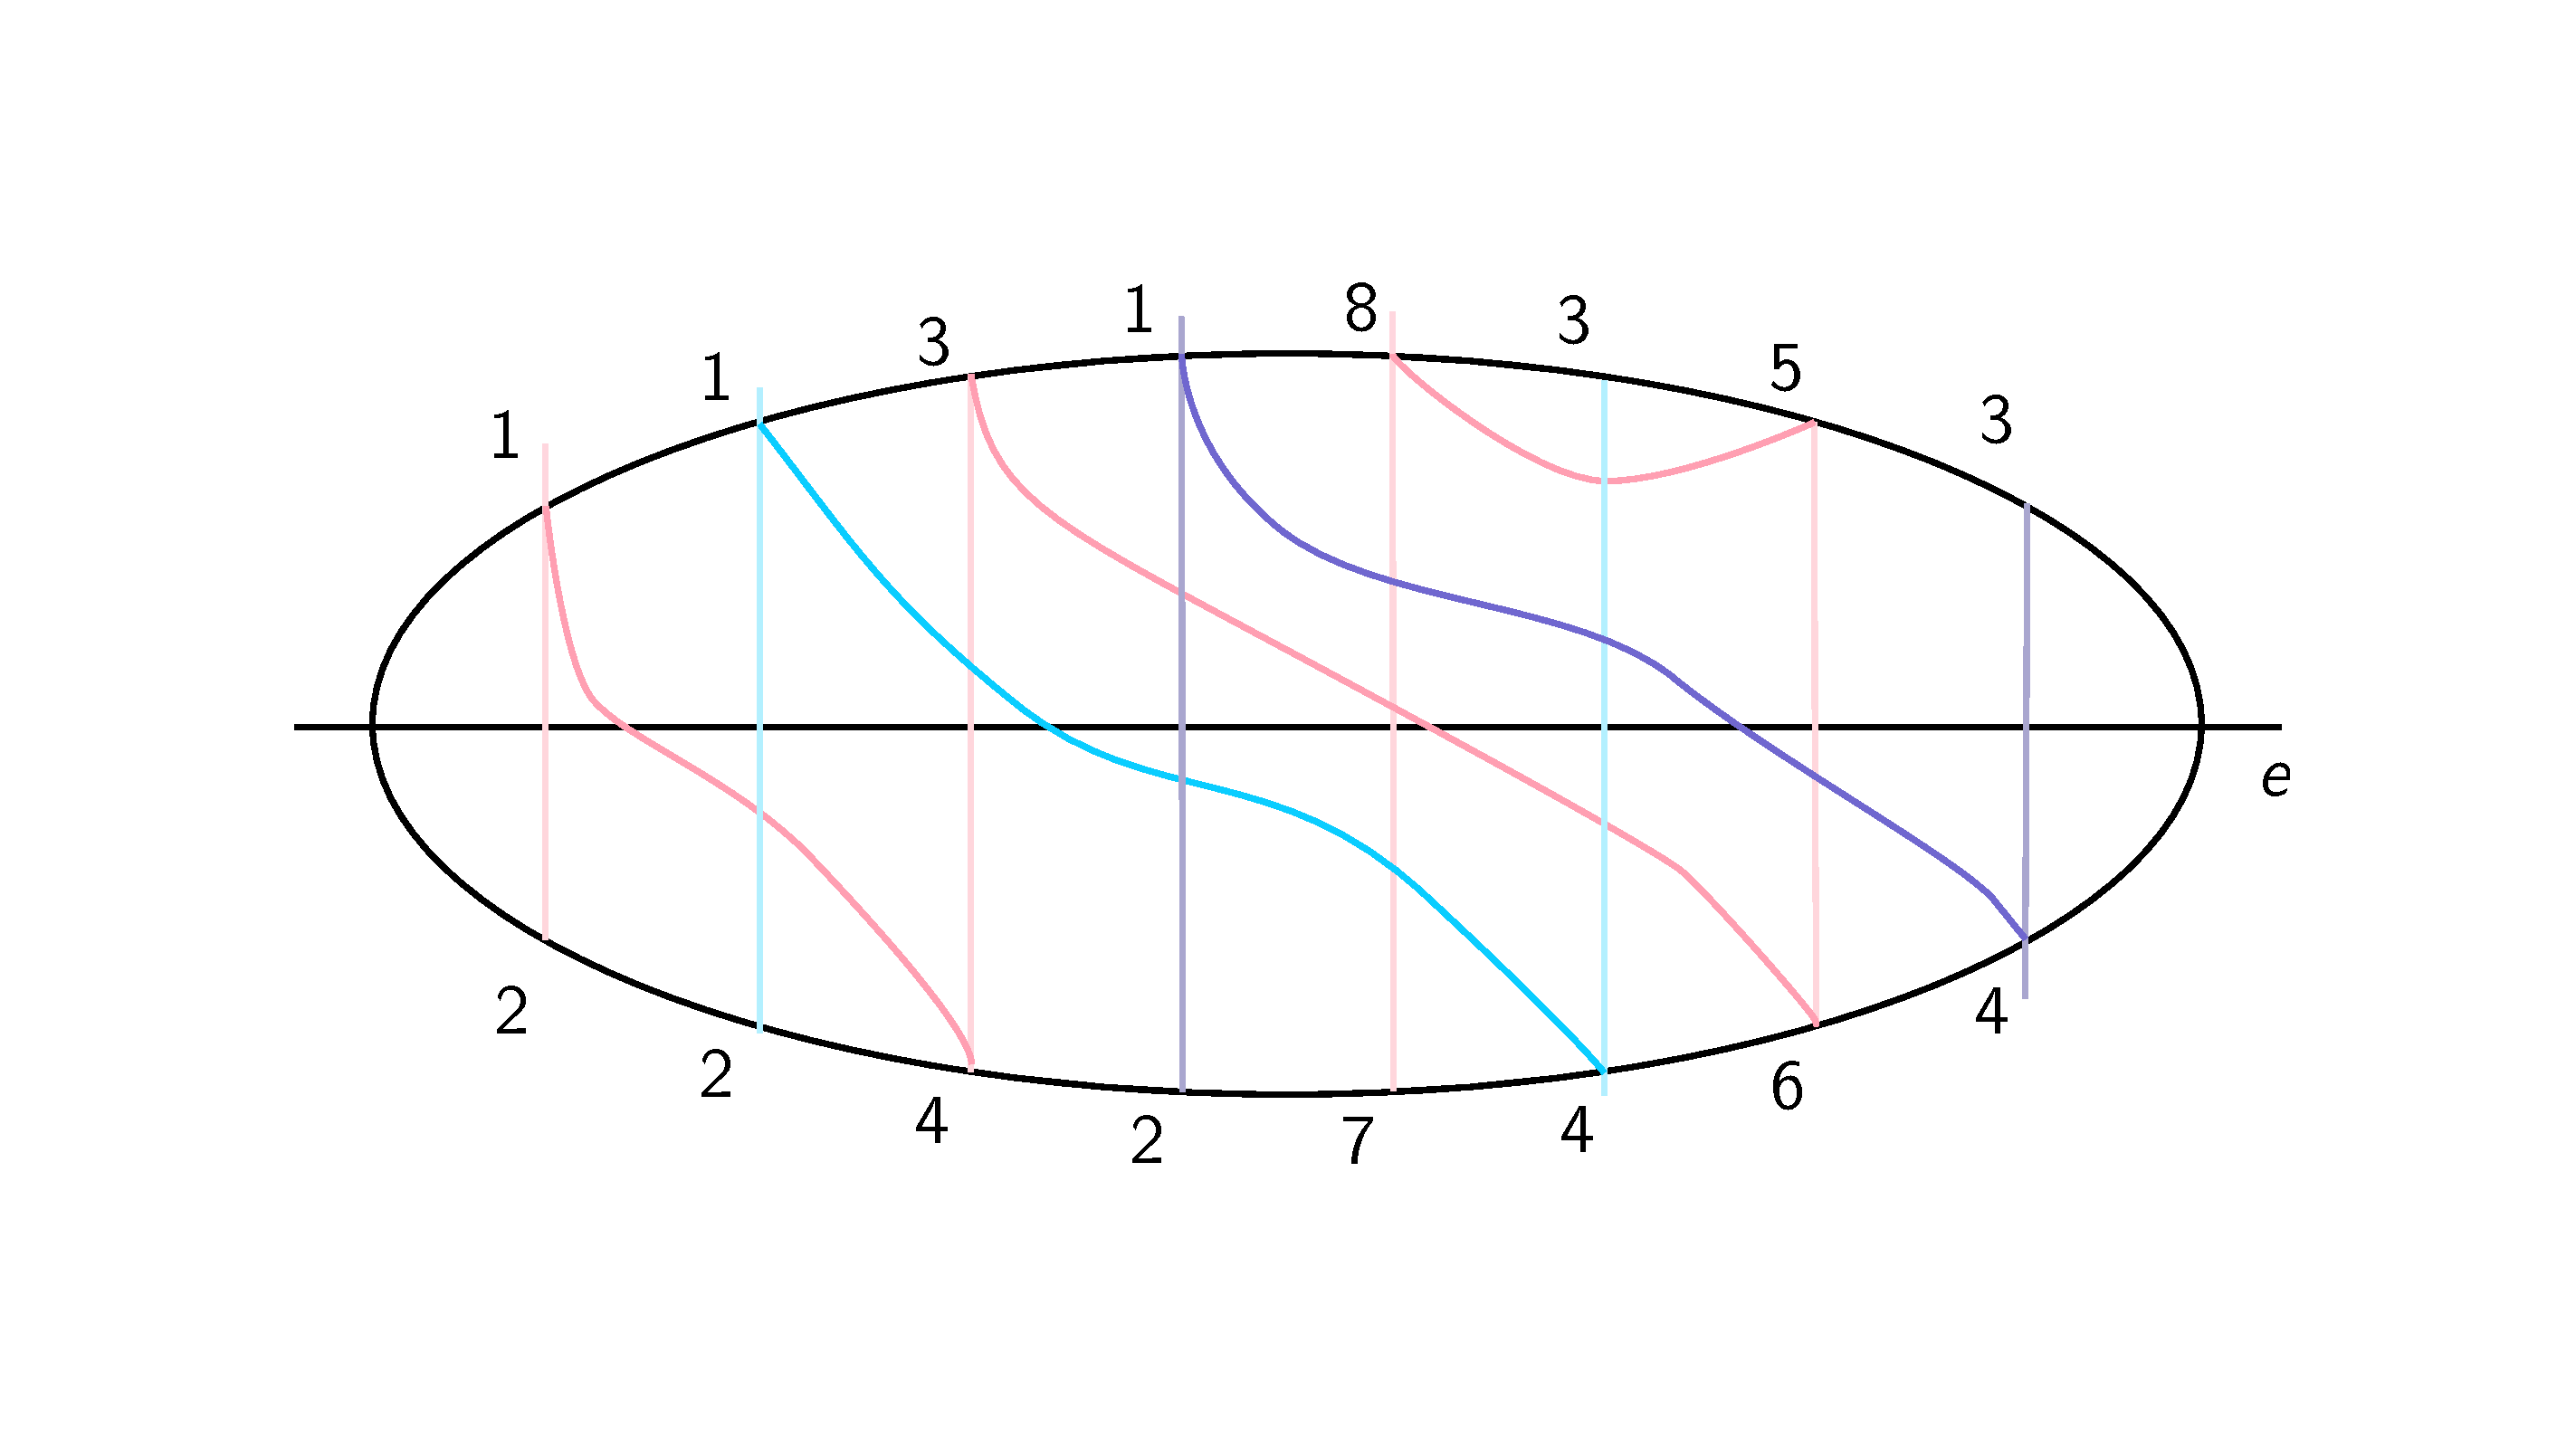
\includegraphics[width=\textwidth]{images/figure-8.pdf}
        \end{center}
    \end{column}
    \end{columns}
\end{frame}

\begin{frame}{Bounding the Number of Intersections 8}
    \begin{columns}
    \begin{column}{0.35\textwidth}
        \begin{itemize}
            \item Now, we have for every edge a connection between \(4i-3\) and \(4i\) which is inside the window.
            \item<2-> Build a new version \(\tilde{f}\): start at intersection \(1\) (connected to one of the endpoints of \(f\)), continue to \(4\) (inside), \(5\) (outside), etc. until \(4 n_f\).            
        \end{itemize}
    \end{column}
    \begin{column}{0.65\textwidth}
        \begin{center}
            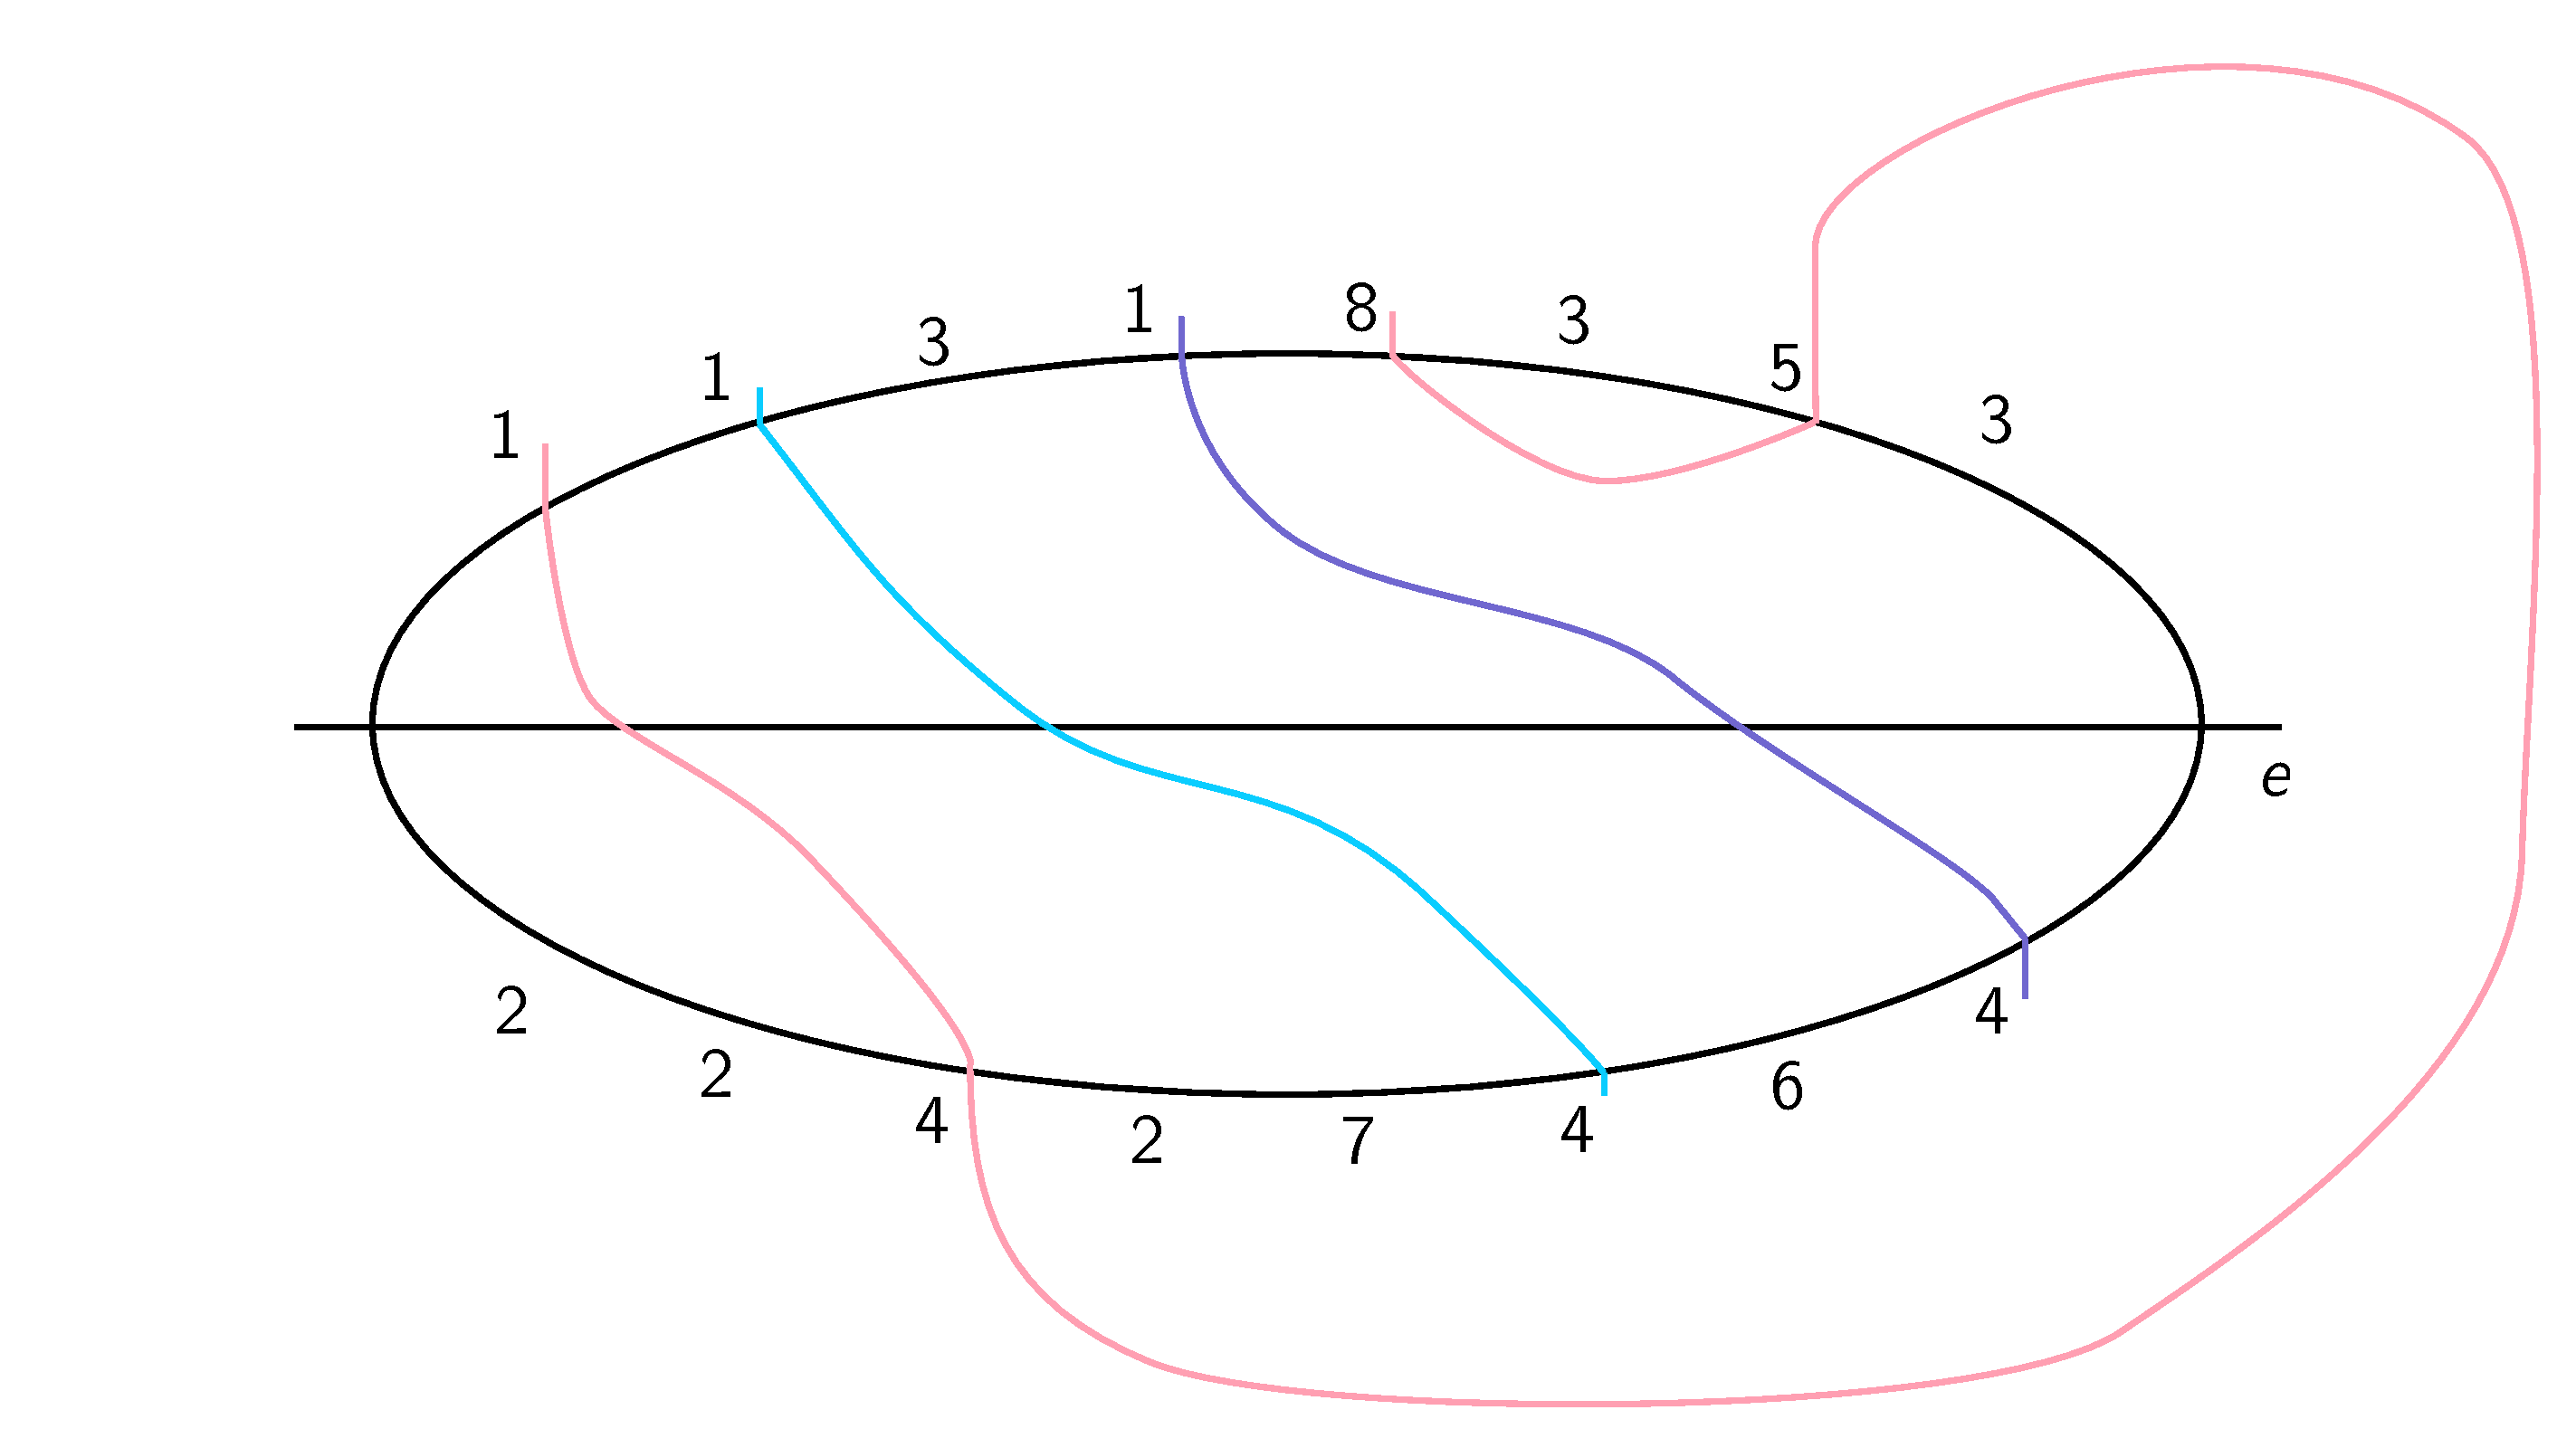
\includegraphics[width=\textwidth]{images/figure-9.pdf}
        \end{center}
    \end{column}
    \end{columns}
\end{frame}

\begin{frame}{Bounding the Number of Intersections 9}
    \begin{columns}
    \begin{column}{0.35\textwidth}
        \begin{itemize}
            \item \(f\) intersects \(e\) an even number of times \(\Rightarrow \tilde{f}\) still connects the two original endpoints.
            \item<2-> \(\leadsto\) reduced the number of intersections with the window from \(4 n_f\) to \(2 n_f\).
            \item<3-> Every intersection between the curves inside the circle corresponds to an intersection outside \(\Rightarrow\) the new realization respects \(R\) (in this example, there are no intersections).
        \end{itemize}
    \end{column}
    \begin{column}{0.65\textwidth}
        \begin{center}
            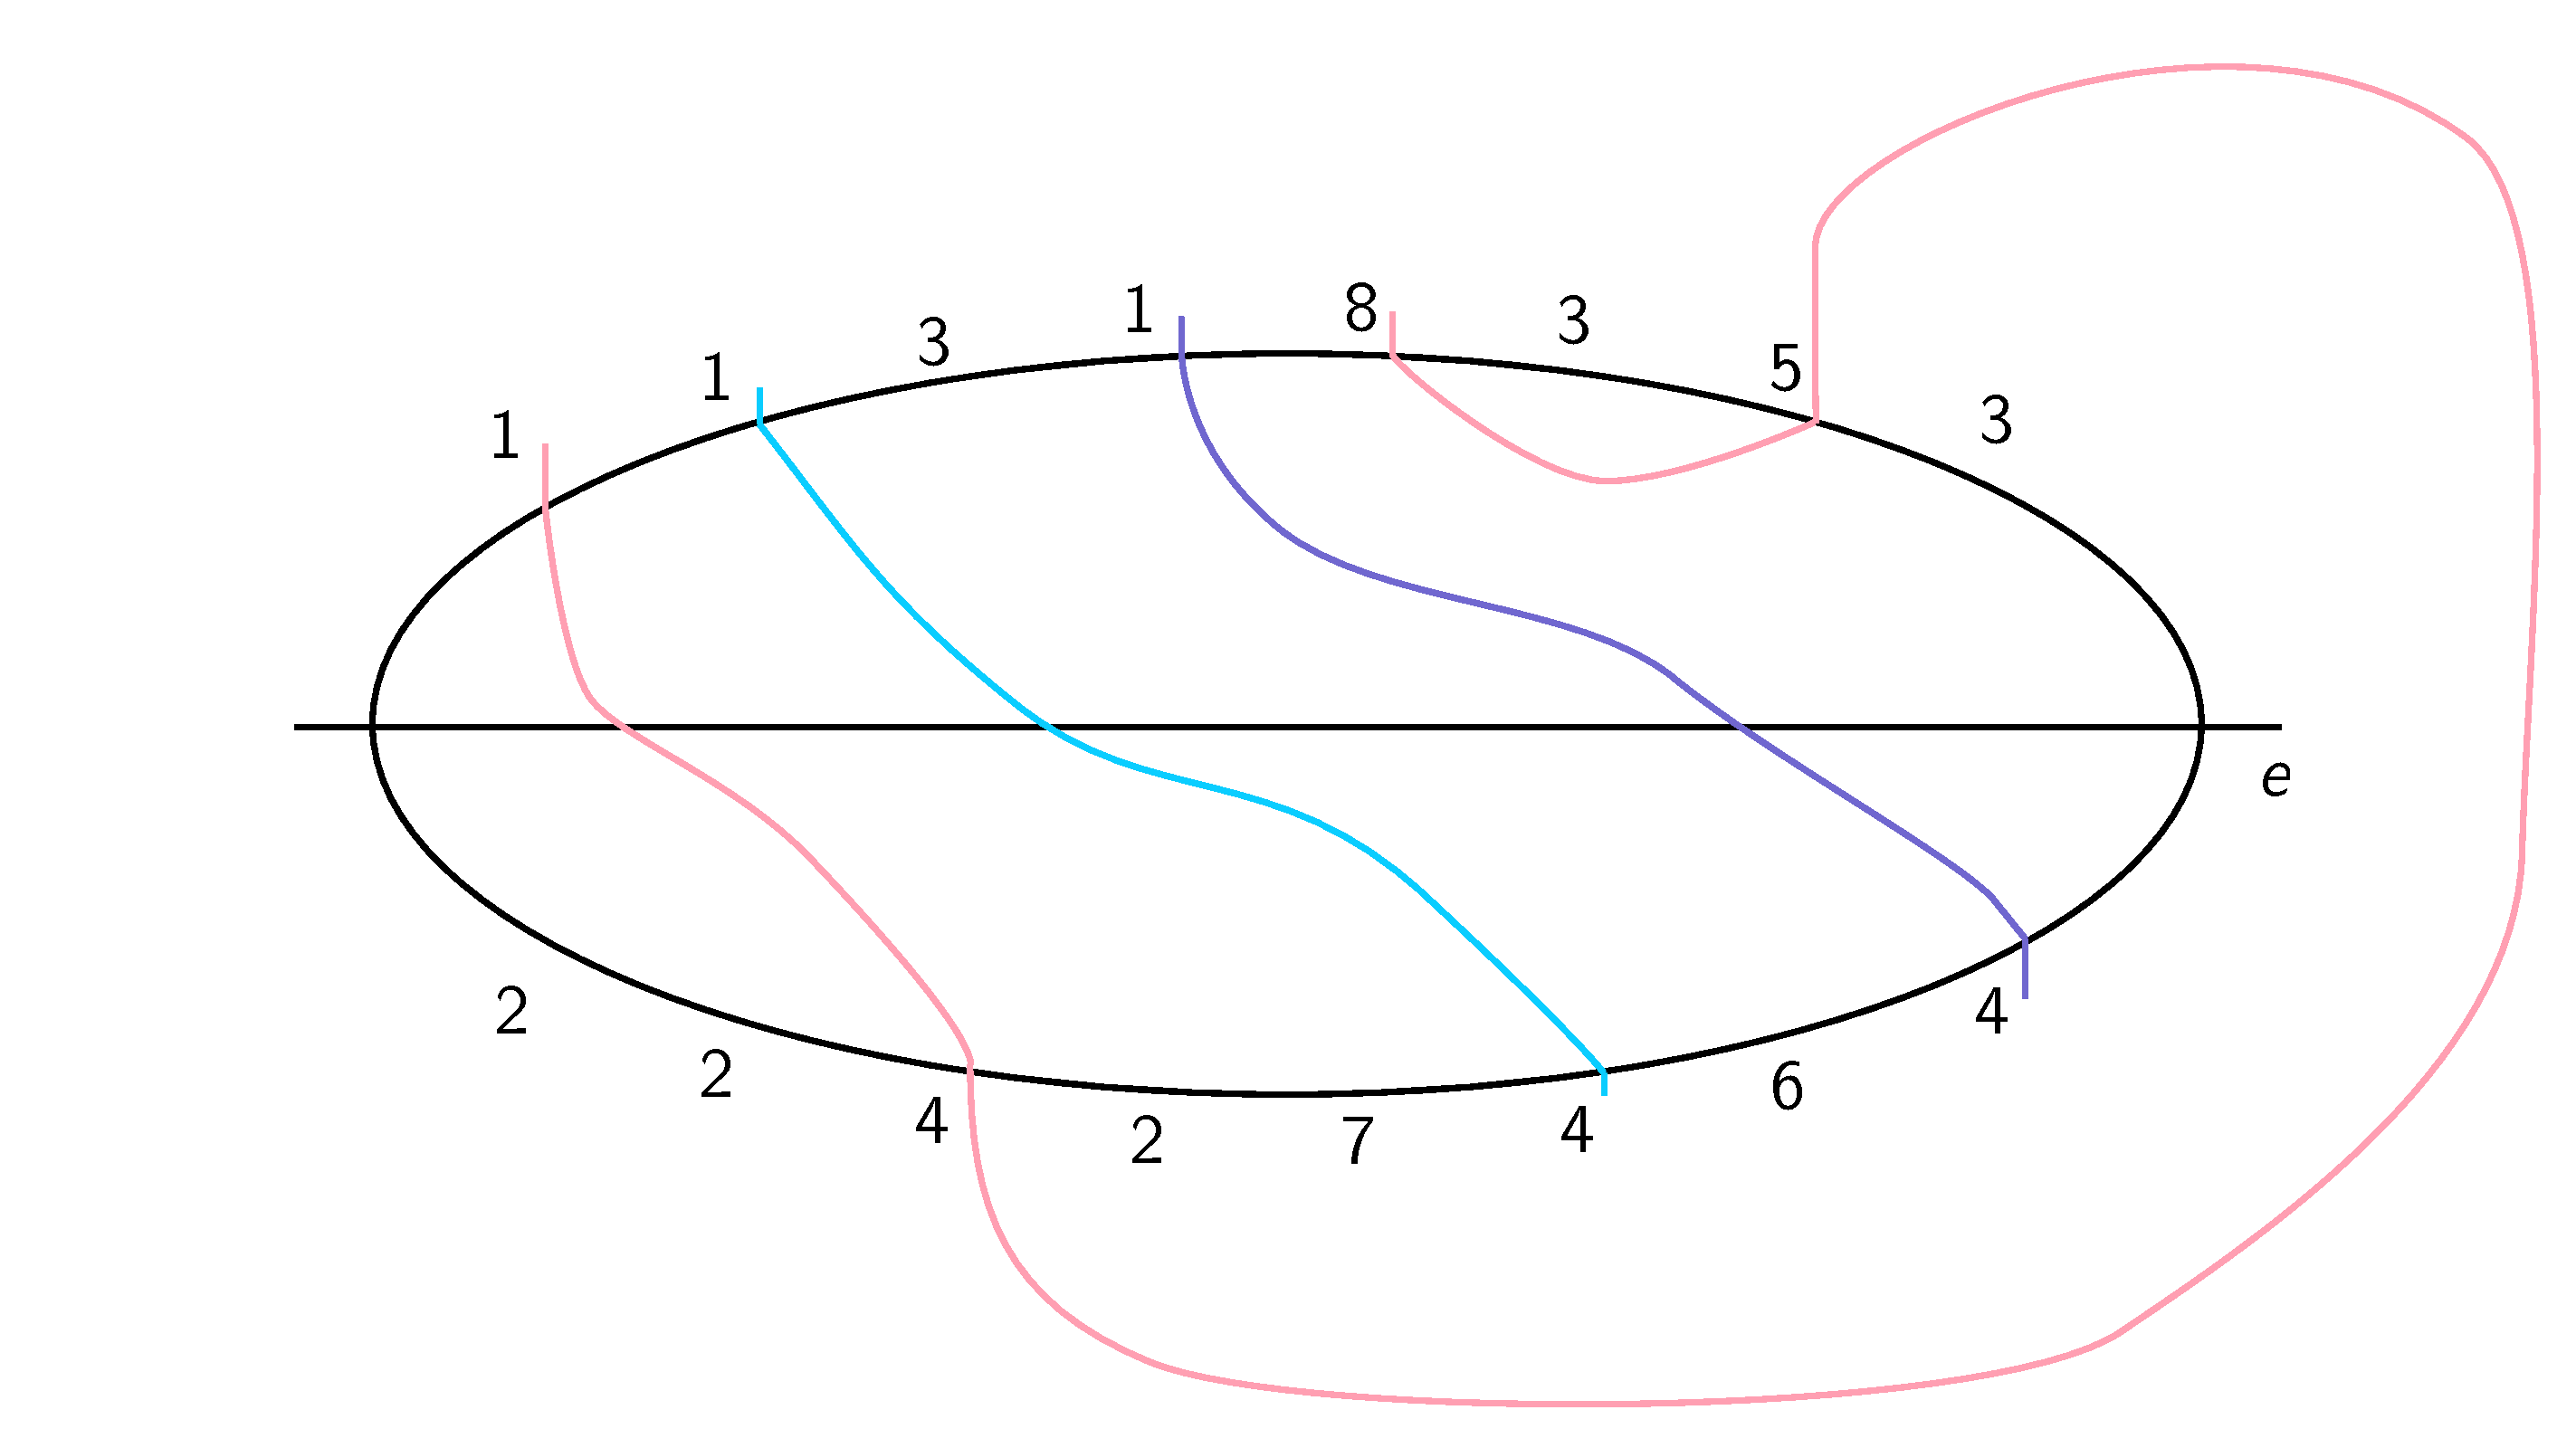
\includegraphics[width=\textwidth]{images/figure-9.pdf}
        \end{center}
    \end{column}
    \end{columns}
\end{frame}

\begin{frame}{Bounding the Number of Intersections 10}
    \begin{columns}
    \begin{column}{0.35\textwidth}
        \begin{itemize}
            \item The number of intersections along \(e\) might have increased.
            \item<2-> \(\tilde{f}\) halved the number of intersections between the intersections and the boundary. 
            \item<3-> \(\leadsto\) \(e'\) = one of the two sides of the boundary of the window (at least one side has less intersections than before).
        \end{itemize}
    \end{column}
    \begin{column}{0.65\textwidth}
        \begin{center}
            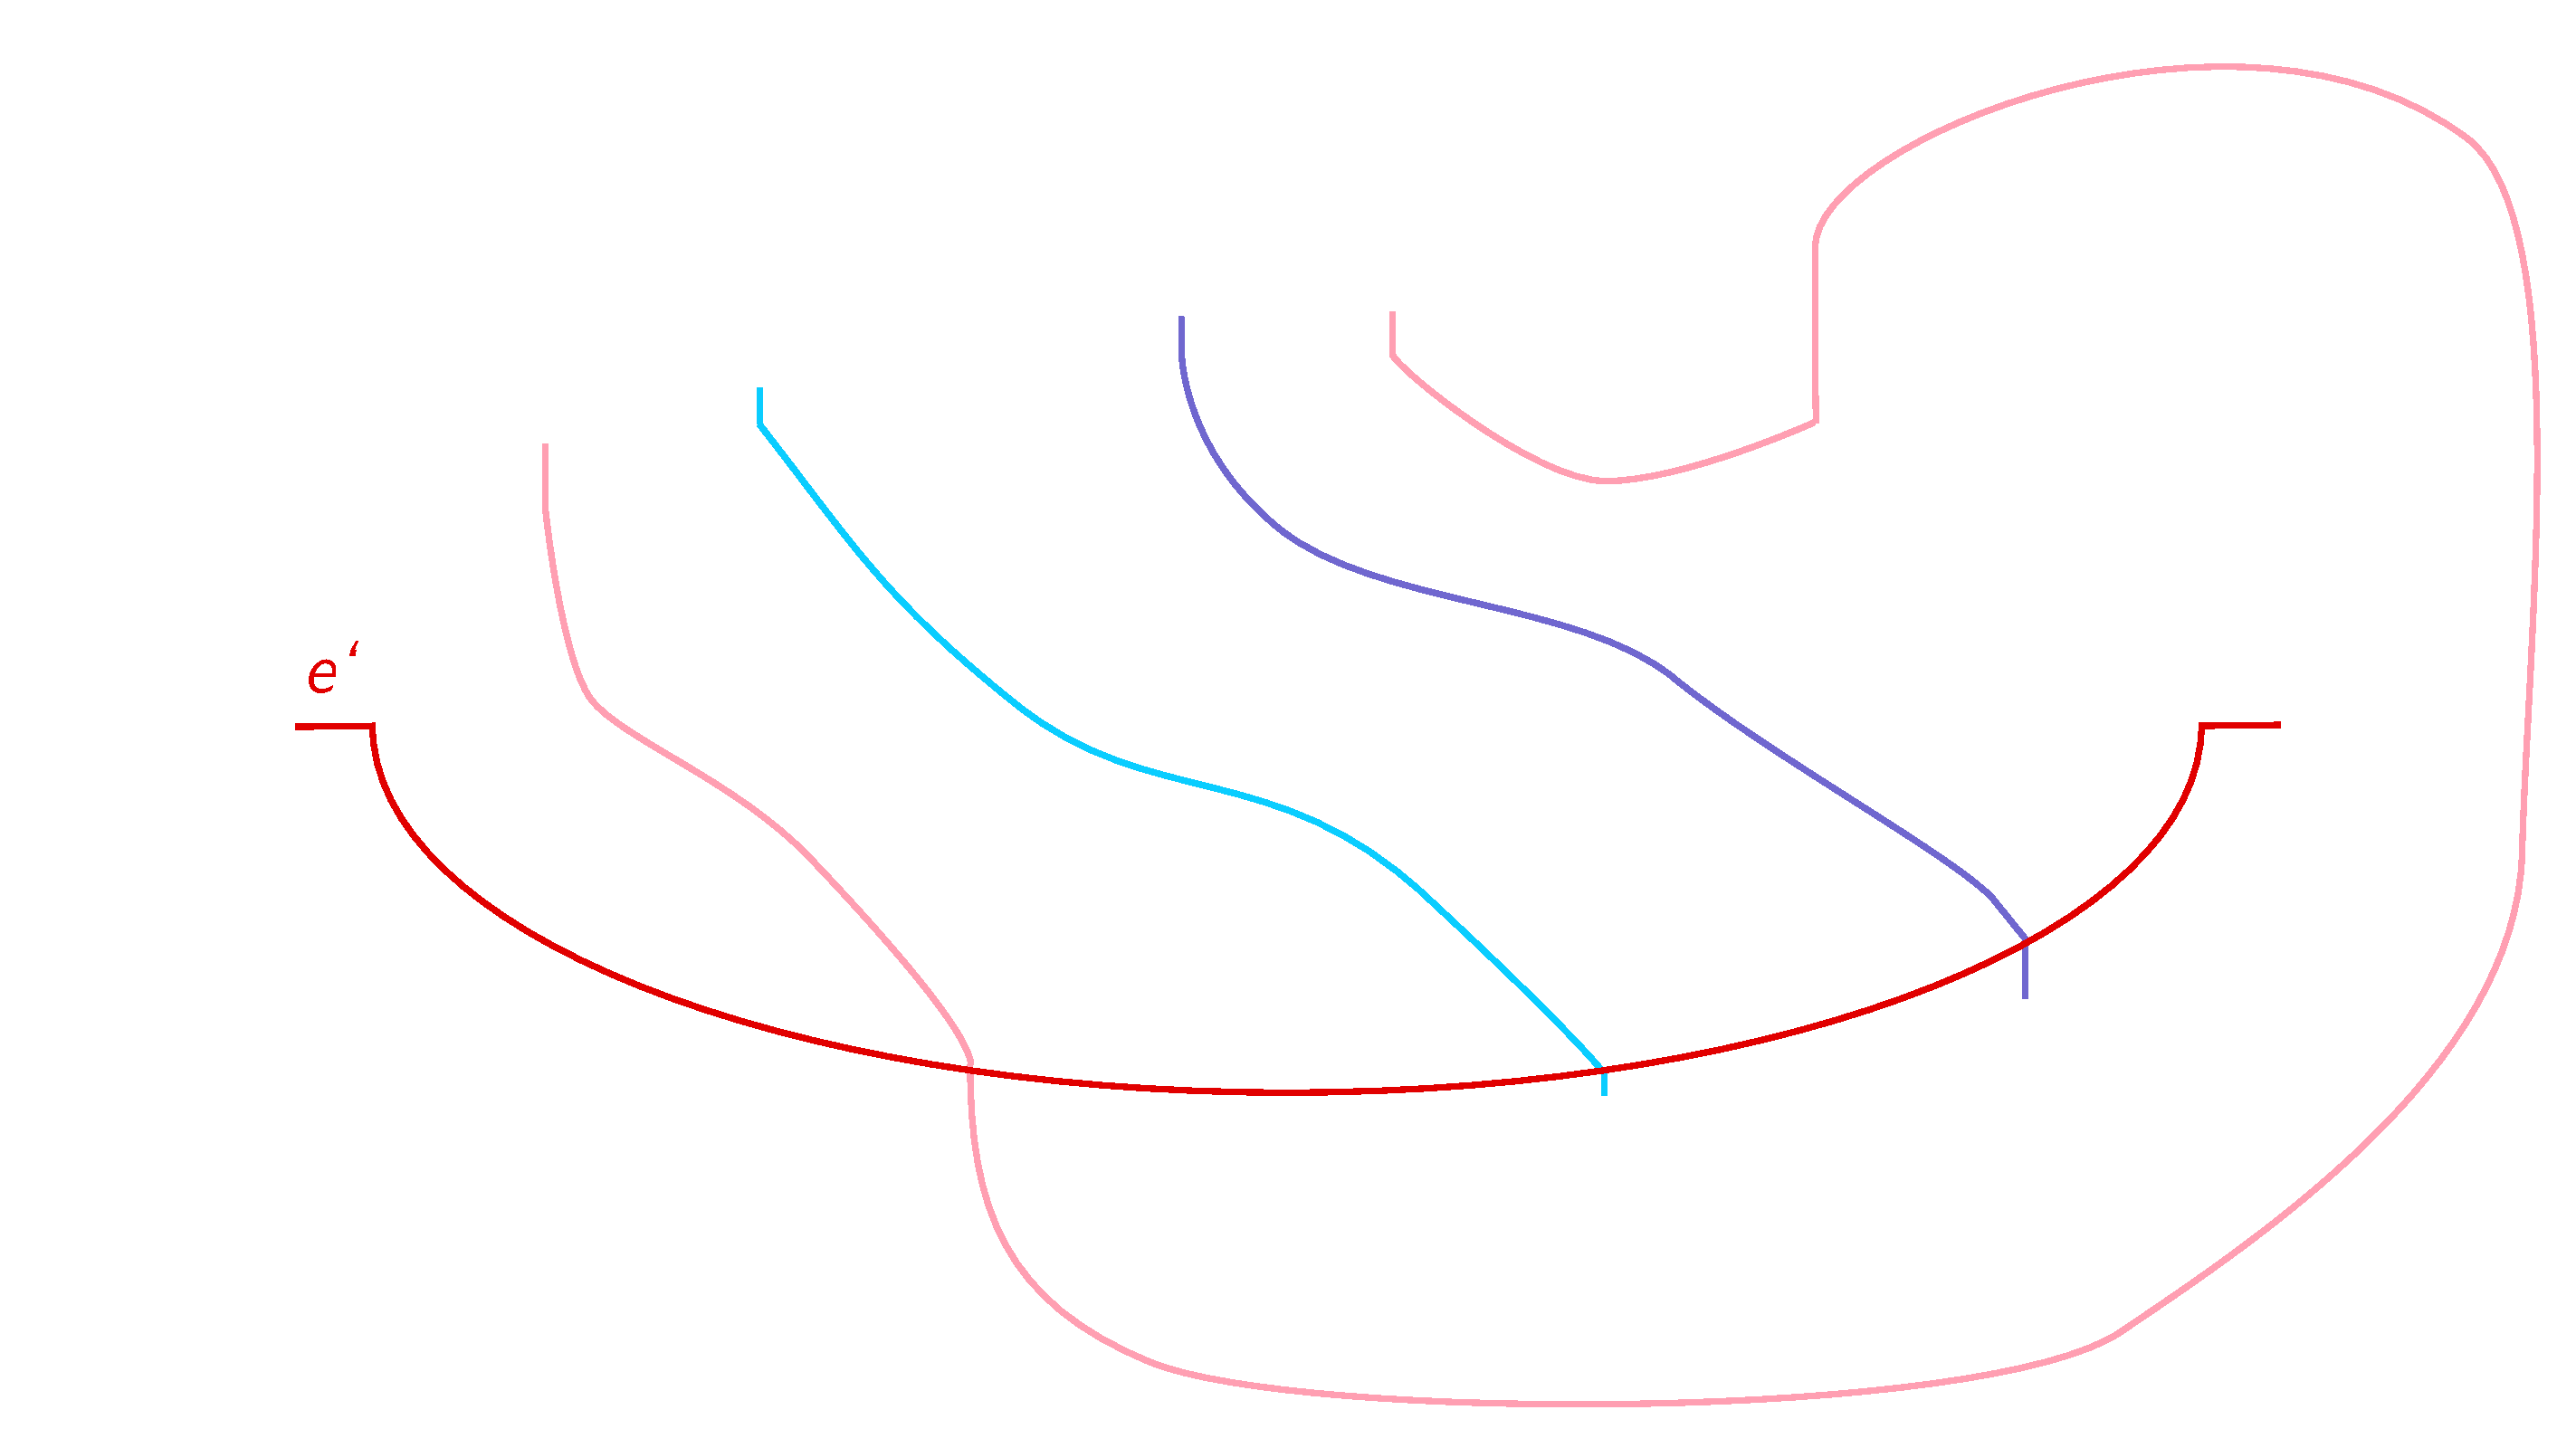
\includegraphics[width=\textwidth]{images/figure-10.pdf}
        \end{center}
    \end{column}
    \end{columns}
\end{frame}

\begin{frame}{String graph decidability}
    \begin{corollary}
        String graph recognition is in \(\mathbf{NEXP}\).
        \label{cor:decidability}
    \end{corollary}
    \begin{theorem}[Schnyder]
        Each plane graph with \(n \geq 3\) vertices has a straight line embedding on the \(n-2\) by \(n-2\) grid.
    \end{theorem}
\end{frame}

\setbeamertemplate{background}[grid]
\addtocounter{theorem}{-2}
\begin{frame}[t]{Corollary \ref{cor:decidability} Proof}
    \begin{corollary}
        String graph recognition is in \(\mathbf{NEXP}\).
    \end{corollary}
    \begin{theorem}[Schnyder]
        Each plane graph with \(n \geq 3\) vertices has a straight line embedding on the \(n-2\) by \(n-2\) grid.
    \end{theorem}
\end{frame}
\setbeamertemplate{background}[default]

\section{String Graphs Requiring Exponential Representations}

\begin{frame}{String Graphs Requiring Exponential Representations}
    Goal: provide a construction of a graph on \(O(n)\) vertices which can be represented
    as a string graph but every realization of the graph requires an exponential number of intersections.

    \(\leadsto\) for string graph testing, we need to check at least exponentially many realizations
\end{frame}

\begin{frame}{Exponential Representations}
    \begin{theorem}
        \(c_w(m) \geq 2^{c m}\) for some constant \(c > 0\).
        \label{thm:exp-cw}
    \end{theorem}
\end{frame}

\setbeamertemplate{background}[grid]
\addtocounter{theorem}{-1}
\begin{frame}[t]{Theorem \ref{cor:exp-cw} Proof}
    \begin{theorem}
        \(c_w(m) \geq 2^{c m}\) for some constant \(c > 0\).
    \end{theorem}
\end{frame}
\setbeamertemplate{background}[default]

\begin{frame}{Exponential Representations}
\includegraphics<1>[width=0.8\textwidth]{images/figure-11.png}\includegraphics<2>[width=0.8\textwidth]{images/figure-12.png}
\end{frame}

\begin{frame}{Exponential Representations}
    \begin{corollary}
        \(c_s(m) \geq 2^{\hat{c} m}\) for some constant \(\hat{c} > 0\).
        \label{cor:exp-cs}
    \end{corollary}
\end{frame}

\setbeamertemplate{background}[grid]
\addtocounter{theorem}{-1}
\begin{frame}[t]{Corollary \ref{cor:exp-cs} Proof}
    \begin{corollary}
        \(c_s(m) \geq 2^{\hat{c} m}\) for some constant \(\hat{c} > 0\).
    \end{corollary}
\end{frame}
\setbeamertemplate{background}[default]

\end{document}
